%% Direttive TeXworks:
% !TeX root = ./semprini_luca_tesi.tex
% !TEX encoding = UTF-8 Unicode
% !TEX program = arara
% !TEX TS-program = arara
% !TeX spellcheck = it-IT

%% Direttive Arara:
% arara: pdflatex: { shell: yes, synctex: yes, action: batchmode, options: "-halt-on-error -file-line-error-style" }
% arara: frontespizio
% arara: biber
% arara: pdflatex: { shell: yes, synctex: yes, action: batchmode, options: "-halt-on-error -file-line-error-style" }
% arara: pdflatex: { shell: yes, synctex: yes, action: nonstopmode, options: "-halt-on-error -file-line-error-style" }

\documentclass[%
    a4paper,        % specifica il formato A4 (default: letter)
    12pt,           % specifica la dimensione del carattere a 12
    openright,      % serve per aprire i capitoli sulla destra
    oneside,        % serve per fare fronteretro
    % draft,        % evidenzia i punti in cui il testo sborda dai margini con delle barre nere, va tolta nella versione definitiva % TODO utile per il controllo
    titlepage       % opzione necessaria per il pacchetto frontespizio
]{book}
\usepackage{a4wide}             % consente di avere più spazio nell'A4
\usepackage[english,italian]{%
    babel,          % serve per scrivere Indice, Capitolo, etc in Italiano
    varioref        % introduce il comando \vref da usarsi nello stesso modo del comune \ref per i riferimenti
} %Where the figures folder is located
\usepackage[T1]{fontenc}        % serve per impostare la codifica di output del font come Latin1 (T1)

%\usepackage{lmodern}           % catica un variante Latin Modern prodotto dal GUST (gruppo utenti di TEX polacco)
%\usepackage{newtxtext}         % insieme a {newtxmath} carica font Times, Times Italic e Helvetica
%\usepackage{newtxmath}         % insieme a {newtxtext} carica font Times, Times Italic e Helvetica
\usepackage{textcomp}           % serve per fornire supporto ai Text Companion fonts
\usepackage[utf8]{inputenc}     % serve per impostare la codifica di input del font come UTF8 (codifica di questo file .tex)
\usepackage{lmodern}            % necessario per risolvere un errore col font, si può usare times o lmodern (o probabilmente anche altro)
\usepackage{listings, chngcntr}           % fondamentale per gli snippet di codice
\usepackage{color}
\usepackage[dvipsnames]{xcolor}
\usepackage{indentfirst}        % serve per avere l'indentazione all'inizio di capitoli, sezioni, etc
\usepackage{setspace}           % serve a fornire comandi di interlinea standard, alternativi a \linespread{}
\usepackage{fancyhdr}           % serve per impaginare bene la tesi
%\usepackage{refcheck}          % serve per controllare l’utilizzo dei \label e dei \ref, va tolta nella versione definitiva    %TODO utile per il controllo
%\usepackage{showkeys}          % serve per mostrare le etichette, va tolta nella versione definitiva                           %TODO utile per il controllo
\usepackage{xcolor}             % serve per la gestione dei colori nel testo
\usepackage{graphicx}           % serve per includere immagini e grafici
%\usepackage{pgfplots}
%\pgfplotsset{compat=1.15}

\renewcommand{\lstlistingname}{Esempio}% Listing -> Esempio

%definizione di alcuni colori
\definecolor{gray}{rgb}{0.4,0.4,0.4}
\definecolor{darkblue}{rgb}{0.0,0.0,0.6}
\definecolor{cyan}{rgb}{0.0,0.6,0.6}
\definecolor{pblue}{rgb}{0.13,0.13,1}
\definecolor{pgreen}{rgb}{0,0.5,0}
\definecolor{pred}{rgb}{0.9,0,0}
\definecolor{pgrey}{rgb}{0.46,0.45,0.48}

%definizione del linguaggio Java per listings
\lstset{language=Java,
  showspaces=false,
  showtabs=false,
  breaklines=true,
  showstringspaces=false,
  breakatwhitespace=true,
  commentstyle=\color{pgreen},
  keywordstyle=\color{pblue},
  stringstyle=\color{pred},
  basicstyle=\ttfamily,
  moredelim=[il][\textcolor{pgrey}]{\$\$},
  moredelim=[is][\textcolor{pgrey}]{\%\%}{\%\%}
}

\lstset{
  basicstyle=\ttfamily,
  columns=fullflexible,
  showstringspaces=false,
  commentstyle=\color{gray}\upshape
}

%definizione del linguaggio XML per listings
\lstdefinelanguage{XML}{
  morestring=[b]",
  morestring=[s]{>}{<},
  morecomment=[s]{<?}{?>},
  stringstyle=\color{black},
  identifierstyle=\color{darkblue},
  keywordstyle=\color{cyan},
  morekeywords={xmlns,version,type}
}
\lstset{
  basicstyle=\scriptsize\sffamily\color{black},
  frame=single,
  numbers=left,
  numbersep=5pt,
  numberstyle=\tiny\color{gray},
  showspaces=false,
  showstringspaces=false,
  tabsize=1
}

%definizione del linguaggio Kotlin per listings
\lstdefinelanguage{Kotlin}{
  keywords={package, as, typealias, this, super, val, var, fun, for, null, true, false, is, in, throw, return, break, continue, object, if, try, else, while, do, when, yield, typeof, yield, typeof, data, class, interface, enum, object, override, public, private, get, set, import, abstract, ->, infix, it, operator, suspend },
  keywordstyle=\color{NavyBlue}\bfseries,
  ndkeywords={@Deprecated, @Test, ReplaceWith, Iterable, Int, Integer, Float, Double, String, Boolean, View, ViewHolder, Runnable, dynamic},
  ndkeywordstyle=\color{BurntOrange}\bfseries,
  emph={println, return@, forEach,},
  emphstyle={\color{OrangeRed}},
  identifierstyle=\color{black},
  sensitive=true,
  commentstyle=\color{gray}\ttfamily,
  comment=[l]{//},
  morecomment=[s]{/*}{*/},
  stringstyle=\color{ForestGreen}\ttfamily,
  morestring=[b]",
  morestring=[s]{"""*}{*"""},
}

\usepackage[htt]{hyphenat}      % Enable hyphenation of TT text
\hyphenation{                   % Permette di sillabare bene le parole
    Kotlin
    Script
    script
    Pack-age
    pack-age
    Manage-ment
    manage-ment
    Com-munity
    com-munity
}

\setcounter{secnumdepth}{2}     % Numera fino alla sottosezione nel corpo del testo
\setcounter{tocdepth}{3}        % Numera fino alla sotto-sottosezione nell'indice


\usepackage[%
    write,          % alternativa a nowrite, crea il file *-frn.tex
    %nowrite,       % alternativa a write, non crea il file *-frn.tex
    standard,       % alternativa a suftesi, crea un frontespizio standard
    %signatures,    % lascia fra i nomi dei relatori lo spazio per le loro firme
    %noadvisor,     % opzione per non mostrare il relatore
    swapnames,      % scambia la posizione dei nomi di relatori e candidato
    normal          % alternativa a sans, utilizza un font "normale"
    %sans,          % alternativa a normal, utilizza un font senza grazie
    %norules,       % eliminano i filetti fra il nome dell’ateneo e quello della facoltà e sopra l’indicazione dell’anno accademico
    %nouppercase,   % disabilita il maiuscoletto nel nome della facoltà
    %noinputenc,    % disabilita la trascrizione dell'inputenc nel preambolo
    %onlyinclude    % disabilita tutte le altre opzioni
]{frontespizio}                 % serve a costruire un buon frontespizio
%\usepackage{fncychap}          % serve a personalizzare il formato dei titoli dei capitoli
%\usepackage[]{titlesec}        % una volta definito lo stile nel preambolo con \titleformat formatta i \chapter{}
%\usepackage{enumitem}          % serve a personalizzare liste enumerate, itemize e description
%\usepackage{minitoc}           % serve a creare mini-indici all'inizio di capitoli particolarmente complessi
%\usepackage{epigraph}          % serve a creare epigrafi
%\usepackage{amssymb}           % abilita i font matematici forniti dall’American Mathematical Society, carica anche {amsfonts}
%\usepackage{mathtools}         % carica {amsmath} e fornisce estensioni per il miglioramento della struttura informativa e della stampa fi formule matematiche
%\usepackage{relsize}           % consente di assegnare dimensioni relative con i comandi \smaller e \larger
%\usepackage{latexsym}
\usepackage[%
    strict,             % rende tutti gli warning degli errori
    autostyle,          % imposta lo stile in base al linguaggio specificato in babel
    english=american,   % imposta lo stile per l'inglese
    italian=guillemets  % imposta lo stile per l'italiano
]{csquotes}                     % serve a impostare lo stile delle virgolette
\usepackage[%
    maxcitenames=2,     % massimo numero di nomi nelle citazioni
    mincitenames=2,     % minimo numero di nomi nelle citazioni
    maxbibnames=99,     % massimo numero di nomi nella blibliografia
    minbibnames=99,     % minimo numero di nomi nella blibliografia
    style=numeric,      %
    giveninits=true,    %
    backend=biber       % specifica il backend per la bibliografia
]{biblatex}                     % si interfaccia con bibtex e biber per la bibliografia
\addbibresource{biblio.bib}
\usepackage[%
    %notbib,            % rimuove la bibliografia dall'indice
    notindex,           % rimuove l'indice dall'indice
    nottoc,             % rimuove la Table of Contents dall'indice
    notlot,             % rimuove la lista delle tabelle dall'indice
    notlof,             % rimuove la lista delle figure dall'indice
    %chapter,           % "Use chapter-level headings, if possible"
    %section,           % "Use section-level headings, if possible"
    %numbib             % numera il capitolo della bibliografia
    %numindex           % numera il capitolo dell'indice
]{tocbibind}

\onehalfspacing                 % Imposta interlinea a 1,5 ed equivale a \linespread{1,5}

%% Bel layout con Fancy
\pagestyle{fancy}\addtolength{\headwidth}{20pt}
\renewcommand{\chaptermark}[1]{\markboth{\thechapter.\ #1}{}}
\renewcommand{\sectionmark}[1]{\markright{\thesection \ #1}{}}
\cfoot{}

\rhead[\fancyplain{}{\bfseries\leftmark}]{\fancyplain{}{\bfseries\thepage}}
\lhead[\fancyplain{}{\bfseries\thepage}]{\fancyplain{}{\bfseries\rightmark}}


\newenvironment{abstract}%
    {\clearemptydoublepage%
        \thispagestyle{empty}%
        \null \vfill\begin{center}%
            \bfseries \phantomsection%
            \addcontentsline{toc}{chapter}{\abstractname}%
            \abstractname \end{center}}%
    {\vfill\null}



\setcounter{secnumdepth}{2}     % Numera fino alla sottosezione nel corpo del testo
\setcounter{tocdepth}{3}        % Numera fino alla sotto-sottosezione nell'indice
%\pdfoptionpdfminorversion=7    % TODO Dovrebbe risolvere il problema di inclusione di pdf 1.5 in 1.4, ma non funziona

%\usepackage[a-1b]{pdfx}        % Permette di generare PDF/A con specifica 1b, TODO verificare
% La chiamata deve essere ritardata il più possibile, ma deve essere prima di hyperref

\usepackage{hyperxmp}           % Simile ad hyperref
\usepackage{hyperref}           % Gestisce tutte le cose ipertestuali del pdf
\hypersetup{%
    pdfpagemode={UseOutlines},
    hidelinks,          % nasconde i collegamenti (non vengono quadrettati)
    hypertexnames=false,
    linktoc=all,        % inserisce i link nell'indice
    bookmarks=true,
    bookmarksopen,
    bookmarksopenlevel=3,
    plainpages=false,
    breaklinks,
    pdfstartview={FitH},
    pdfauthor={Luca Semprini},
    pdfcopyright={Copyright (C) 2017, Luca Semprini},
    pdftitle={Una panoramica su Kotlin: il nuovo linguaggio per lo sviluppo di applicazioni Android},
    pdfcontactcountry={Italy},
    pdfcontactemail={luca.semprini10@studio.unibo.it},
    pdflang={it},
    pdfsubject={Lo scopo della presente tesi di laurea è quello di presentare in maniera esaustiva ed approfondita le caratteristiche e le peculiarità fondamentali del linguaggio di programmazione Kotlin, con particolare attenzione alle sue applicazioni per lo sviluppo di sistemi Android. Il lavoro svolto ha riguardato in primis l'apprendimento del linguaggio e lo studio della sua evoluzione nel tempo, oltre che all'analisi approfondita di tutte le sue sfaccettature e la raccolta delle opinioni degli esperti. Si è continuato organizzando la stesura in maniera originale, cercando di seguire una linea coerente con l'intenzione di toccare in maniera graduale tutti gli argomenti più significativi che riguardassero il liguaggio in questione. Gli esempi di codice forniti nel corso dell'elaborato sono atti a contribuire in maniera sistematica alla presentazione del linguaggio e sono stati concepiti in maniera da risultare sufficientemente esplicativi, sulla base dell'esperienza personale con il linguaggio analizzato.},
    pdfkeywords={Kotlin, Android, Java},
    pdfa
}
\usepackage[all]{hypcap}        % sistema i problemi di hyperref

% cleveref va anche dopo hyperref
\usepackage[%
    english,italian,    % definizione delle lingue da usare
    nameinlink          % inserisce i link nei riferimenti
]{cleveref}                     % permette di usare riferimenti migliori dei \ref e dei varioref

\begin{document}
    \frontmatter
    \pagenumbering{Roman}
    \pagestyle{empty}
    %% Direttive TeXworks:
% !TeX root = ../semprini_luca_tesi.tex
% !TEX encoding = UTF-8 Unicode
% !TEX program = arara
% !TEX TS-program = arara
% !TeX spellcheck = it-IT

%% Direttive Arara:
% arara: pdflatex: { shell: yes, synctex: yes, action: batchmode, options: "-halt-on-error -file-line-error-style" }
% arara: frontespizio
% arara: biber
% arara: pdflatex: { shell: yes, synctex: yes, action: batchmode, options: "-halt-on-error -file-line-error-style" }
% arara: pdflatex: { shell: yes, synctex: yes, action: nonstopmode, options: "-halt-on-error -file-line-error-style" }

\begin{frontespizio}
    \Universita{Bologna}
        \Istituzione{%
            Alma Mater Studiorum - Università di Bologna \\%
            Campus di Cesena%
        }
        \Divisione{Scuola di Scienze}
        \Corso[Laurea]{Ingegneria e Scienze Informatiche}
        \Annoaccademico{2016-2017}
        % \Titoletto{Tesi di laurea}
        \Titolo{%
            Kotlin: un nuovo linguaggio \\%
            per lo sviluppo di applicazioni \\%
            Android%
        }
        \Sottotitolo{Tesi in Programmazione ad Oggetti}
        \Candidato{Luca~Semprini}
        \NCandidato{Presentata da}
        \Relatore{Prof.~Mirko~Viroli}
        \Piede{%
            II sessione di laurea \\%
            Anno Accademico 2016 - 2017%
        }
    \end{frontespizio}

    %% Direttive TeXworks:
% !TeX root = ../../semprini_luca_tesi.tex
% !TEX encoding = UTF-8 Unicode
% !TEX program = arara
% !TEX TS-program = arara
% !TeX spellcheck = it-IT

%% Direttive Arara:
% arara: pdflatex: { shell: yes, synctex: yes, action: batchmode, options: "-halt-on-error -file-line-error-style" }
% arara: frontespizio
% arara: biber
% arara: pdflatex: { shell: yes, synctex: yes, action: batchmode, options: "-halt-on-error -file-line-error-style" }
% arara: pdflatex: { shell: yes, synctex: yes, action: nonstopmode, options: "-halt-on-error -file-line-error-style" }
\newcommand{\clearemptydoublepage}{\newpage{\pagestyle{empty}%
    \cleardoublepage}}
\clearemptydoublepage
\thispagestyle{empty}
\vspace*{20ex}
\begin{flushright}
    \begin{LARGE}
        \textbf{Parole chiave}\\
        \vspace{5ex}
    \end{LARGE}
    \begin{normalsize}
        \textbf{%
            Kotlin\\%
            %
            % %
            %
            Android\\%
            \medskip
            % Java
            % \medskip
            %
            %\medskip
            %
        }
    \end{normalsize}
\end{flushright}
\vfill
\clearemptydoublepage

    % %% Direttive TeXworks:
% !TeX root = ../semprini_luca_tesi.tex
% !TEX encoding = UTF-8 Unicode
% !TEX program = arara
% !TEX TS-program = arara
% !TeX spellcheck = it-IT

\null\vspace{\stretch{1}}
\begin{flushright}

    \textit{Qui ci va la dedica}

\end{flushright}
\vspace{\stretch{2}}\null

    %% Direttive TeXworks:
% !TeX root = ../../semprini_luca_tesi.tex
% !TEX encoding = UTF-8 Unicode
% !TEX program = arara
% !TEX TS-program = arara
% !TeX spellcheck = it-IT

\begin{abstract}
Lo scopo della presente tesi di laurea è quello di presentare in maniera esaustiva ed approfondita le caratteristiche e le peculiarità fondamentali del linguaggio di programmazione Kotlin, con particolare attenzione alle sue applicazioni per lo sviluppo di sistemi Android.\\

La trattazione è strutturata su quattro capitoli: nel \Cref{ch:presentazione} viene illustrato il contesto storico in cui la progettazione del linguaggio ha avuto luogo, nonché le piattaforme target per cui poterlo utilizzare, i concetti fondamentali della filosofia del linguaggio e i principali metodi di compilazione; nel \Cref{ch:sintassi} viene esposta la sintassi basilare del linguaggio e le sue caratteristiche più interessanti, fornendo in maniera sistematica esempi di codice esplicativi;
nel \Cref{ch:android} viene approfondita la piattaforma Android come target principale di Kotlin, fornendo esempi di feature proprie del linguaggio che possono risultare congeniali allo sviluppo di applicazioni in questo ambiente: anch'esse vengono corredate da esempi di codice per un approfondimento ulteriore; in questo capitolo vengono, inoltre, analizzate le prestazioni del linguaggio sotto l'aspetto della velocità di compilazione, del conteggio dei metodi, dell'impatto sulle dimensioni dell'applicazione scritta in Kotlin, e sulla stabilità effettiva di quest'ultima. Infine, nel \Cref{ch:conclusione} viene effettuata un'analisi sullo stato attuale del linguaggio e la sua popolarità, concludendo con una valutazione delle prospettive future in ambito Android che Kotlin potrà riscontrare nei mesi a venire.


\end{abstract}

    \tableofcontents

    \graphicspath{{./img/}}
    \mainmatter
    \pagenumbering{arabic}
    \pagestyle{fancy}
    \counterwithin{lstlisting}{section}
    \counterwithin{figure}{section}
    %% Direttive TeXworks:
% !TeX root = ../semprini_luca_tesi.tex
% !TEX encoding = UTF-8 Unicode
% !TEX program = arara
% !TEX TS-program = arara
% !TeX spellcheck = it-IT

\chapter*{Introduzione}\label{ch:intro}
\addcontentsline{toc}{chapter}{\nameref{ch:intro}}

Il lavoro svolto in questa tesi di laurea ha come obiettivo quello di illustrare ed analizzare le caratteristiche principali del linguaggio di programmazione Kotlin e le sue funzionalità più vantaggiose per lo sviluppo di applicazioni Android.\\

Kotlin è un linguaggio di programmazione orientato agli oggetti staticamente tipizzato che nasce nel 2011, anno del primo annuncio ufficiale, da un team di sviluppatori di JetBrains. Si tratta di un linguaggio prevalentemente improntato su Java, che viene quindi compilato in un byte-code eseguibile sulla Java Virtual Machine; tuttavia, offre la possibilità di essere compilato in JavaScript o in codice nativo, utilizzando la struttura di compilazione LLVM \cite{LLVMWiki}.\\
Kotlin si pone oggi come obiettivo quello di rappresentare una valida alternativa a Java soprattutto nello sviluppo di applicazioni Android, fornendo un sistema di tipi sicuro dal punto di vista della prevenzione di crash durante l'esecuzione e una sintassi moderna, concisa ed elegante, che riprende molti noti costrutti che hanno fatto la fortuna di linguaggi come Scala, Groovy, C\# e Java stesso.\\
La libreria standard di Kotlin si appoggia completamente sul framework Java, estendendolo con funzionalità inedite: questo dimostra la forte interoperabilità tra i due linguaggi.
Kotlin presenta diverse caratteristiche sintattiche di rilievo, tra cui la possibilità di definire funzioni {\em inline}, se costituite da un'unica espressione, che rendono il byte-code generato dal compilatore molto più performante; le data classes sono un costrutto che permette di definire in pochissime linee di codice una classe che fornisca un supporto conveniente per immagazzinare e gestire dati; le funzioni di estensione sono funzioni che possono essere chiamate come membro di una certa classe ma vengono definite al di fuori di essa, permettendo di estendere codice scritto in qualsiasi linguaggio JVM.\\

L'utilizzo di Kotlin per la programmazione di applicazioni Android sta prendendo sempre più piede, grazie a diverse funzionalità che risultano peculiari per questo ambiente di esecuzione, come le Lambda Expressions (simili alle omonime Java, ma più potenti), le Coroutines (che utilizzano i paradigmi più diffusi di programmazione asincrona d C\#, Python, Go e JavaScript) o le Annotazioni. Un'altra importante discriminante che ha reso Kotlin sempre più popolare per lo sviluppo su Android è stato l'annuncio ufficiale da parte di Google di renderlo un linguaggio ufficialmente supportato (e integrato nella IDE ufficiale di programmazione Android Studio).\\

Il lavoro svolto ha riguardato in primis l'apprendimento del linguaggio e lo studio della sua evoluzione nel tempo, oltre che all'analisi approfondita di tutte le sue sfaccettature e la raccolta delle opinioni degli esperti. Si è continuato organizzando la stesura in maniera originale, cercando di seguire una linea coerente con l'intenzione di toccare in maniera graduale tutti gli argomenti più significativi che riguardassero il liguaggio in questione. Gli esempi di codice forniti nel corso dell'elaborato sono atti a contribuire in maniera sistematica alla presentazione del linguaggio e sono stati concepiti in maniera da risultare sufficientemente esplicativi, sulla base dell'esperienza personale con il linguaggio analizzato.\\

    %% Direttive TeXworks:
% !TeX root = ../semprini_luca_tesi.tex
% !TEX encoding = UTF-8 Unicode
% !TEX program = arara
% !TEX TS-program = arara
% !TeX spellcheck = it-IT

%% Direttive Arara:
% arara: pdflatex: { shell: yes, synctex: yes, action: batchmode, options: "-halt-on-error -file-line-error-style" }
% arara: frontespizio
% arara: biber
% arara: pdflatex: { shell: yes, synctex: yes, action: batchmode, options: "-halt-on-error -file-line-error-style" }
% arara: pdflatex: { shell: yes, synctex: yes, action: nonstopmode, options: "-halt-on-error -file-line-error-style" }
\chapter{Presentazione del linguaggio Kotlin}
Kotlin è un linguaggio di programmazione a tipizzazione statica e forte, principalmente improntato su Java,
quindi sul paradigma Object-Oriented, ma con importanti funzionalità proprie dei linguaggi funzionali.
Essendo pensato per interoperare con il codice Java, viene eseguito sulla Java Virtual Machine,
ma può anche essere compilato nel codice sorgente di JavaScript o utilizzando la struttura di compilazione LLVM
(Low Level Virtual Machine). Il suo sistema Object-Oriented, come quello di Java, è basato sull'ereditarietà
singola a livello di classe e sull'eredità multipla a livello di interfaccia. Solo le classi possono contenere dati e il codice di inizializzazione, mentre le interfacce possono contenere membri funzionali astratti e, eventualmente, loro predefinite implementazioni. Il suo sistema di tipi è basato su sottotipazione nominale (piuttosto che strutturale) con polimorfismo sottotipato (membri funzionali virtuali), con il supporto di generici - una forma di polimorfismo parametrico con parametri di tipo vincolati, varianza generica e proiezioni di tipo (una semplice forma ristretta dei tipi esistenziali, in qualche modo simili alle Java wildcards).\\

\begin{figure}[htbp]
  \centering
  
\includegraphics[scale=0.05]{logo.png}
  \caption{{\bfseries Logo ufficiale di Kotlin dal febbraio 2016}}
  \label{logoKt}
\end{figure}

\section{Caratteristiche principali}
Come già accennato, proprio come Java, Kotlin è un linguaggio di programmazione staticamente tipizzato.
Questo significa che il tipo di ogni espressione di un programma è noto al momento della compilazione
e il compilatore può inferire che i metodi e i campi a cui si tenta di accedere esistano sugli oggetti
che si sta utilizzando. \\
Ciò è in contrasto con i linguaggi di programmazione dinamicamente tipizzati, che sono
rappresentati nell’ambito JVM da, tra gli altri, Groovy e JRuby. Questi permettono di
definire variabili e funzioni che possono memorizzare o restituire dati di qualsiasi tipo e risolvere metodi
e riferimenti dei campi a runtime: ciò consente un codice più compatto e maggiore
flessibilità nella creazione di strutture di dati. Ma il lato negativo è che i problemi come gli errori
di battitura durante la scrittura degli identificativi delle variabili non possono essere rilevati durante
la compilazione e causano errori di runtime. \\
D'altra parte, contrariamente a Java, Kotlin non richiede di specificare il tipo di ogni variabile
esplicitamente durante la scrittura del codice. In molti casi, il tipo delle variabili può venire
automaticamente determinato dal contesto, consentendo di omettere la dichiarazione di tipo.
La capacità del compilatore di determinare tipi dal contesto è chiamata {\em inferenza di tipo}. \\

Alcuni dei vantaggi della tipizzazione statica sono:
\begin{itemize}
  \item {\bfseries Prestazioni -} I metodi di chiamata sono più veloci perché non c'è bisogno di capire in fase
        di esecuzione quale metodo debba essere effettivamente chiamato.
  \item {\bfseries Affidabilità -} Il compilatore verifica la correttezza del programma, quindi ci sono meno
        possibilità di crash durante il runtime.
  \item {\bfseries Manutenzione -} Lavorare con codice scritto da altri è più semplice e intuitivo, in quanto
        si può vedere con quale tipo di oggetti il codice sta lavorando.
  \item {\bfseries Tool-support -} La tipizzazione statica consente refactoring affidabili, auto completamento
        preciso del codice e altre funzionalità a livello di IDE.
\end{itemize}
Grazie al supporto di Kotlin all'inferenza di tipo, la maggior parte della verbosità aggiuntiva associata
alla tipizzazione statica scompare, perché non è più necessario dichiarare i tipi esplicitamente.
Le classi, le interfacce e i generici funzionano in un modo molto simile a quello di Java, quindi la
maggior parte delle conoscenze di Java, da parte degli sviluppatori, possono essere facilmente “riutilizzate”
nell’apprendimento di Kotlin. Tuttavia, ci sono chiaramente delle novità: la più importante di queste è il sostegno
di Kotlin per i tipi Nullable, che permettono di scrivere programmi più affidabili individuando eventuali
\texttt{NullPointerException} a tempo di compilazione. Un'altra novità nel sistema di tipo di Kotlin è rappresentata
dal suo supporto per i tipi funzionali. Per capire di cosa si tratti, verranno presentate le idee principali
della programmazione funzionale e come essa sia supportata da Kotlin.\\

Per quanto riguarda il paradigma della programmazione funzionale, i concetti chiave che Kotlin introduce sono i seguenti:
\begin{itemize}
  \item {\bfseries First-class functions –} Si lavora con funzioni (blocchi di codice) come valori primari.
        È possibile, infatti, memorizzarle in variabili, passarle come parametri o restituirle da altre funzioni.
  \item {\bfseries Immutabilità –} Si utilizzano oggetti immutabili, ovvero che garantiscono che il loro stato
        interno non cambierà dopo la loro creazione.
  \item {\bfseries Nessun side-effect –} Vengono utilizzate funzioni pure, che restituiscono
        lo stesso risultato dati gli stessi parametri in ingresso e non modificano lo stato di altri oggetti,
        né interagiscono con il mondo esterno.
\end{itemize}
La scrittura del codice nello stile funzionale può portare a diversi benefici.\\
Innanzitutto, giova alla concisione: il codice funzionale può essere più elegante
e sintetico rispetto alla sua controparte imperativa, perché lavorare con funzioni come valori può dare molta di più possibilità di astrazione, che può voler dire evitare la duplicazione nel codice. \\
Un secondo beneficio del codice funzionale è la possibilità di utilizzare proprietà multithreading
in maniera più sicura. Una delle più grandi fonti di errori nei programmi multithreaded consiste
nella modifica degli stessi dati da parte di più thread senza una adeguata sincronizzazione;
utilizzando strutture dati di tipo immutabile e le funzioni pure, si possono facilmente evitare tali errori,
senza dover elaborare schemi di sincronizzazione particolarmente complicati. \\
Infine, la programmazione funzionale può portare alla semplificazione della fase di testing,
infatti, del codice senza effetti collaterali è di solito più facile da testare. \\
In generale, lo stile funzionale può essere utilizzato con qualsiasi linguaggio di programmazione,
tra cui Java, tuttavia non tutti i linguaggi forniscono il supporto sintattico e di libreria
necessario per far sì che ciò avvenga senza sforzo; ad esempio, questo supporto è mancato molto
nelle versioni di Java prima di Java 8. \\
Kotlin ha un ricco set di funzionalità per supportare la programmazione funzionale, tra cui:
\begin{itemize}
  \item Tipi funzionali, che consentono alle funzioni di ricevere altre funzioni come parametri o di ritornare altre funzioni.
  \item Le Lambda expressions permettono di passare blocchi di codice con un minimo boilerplate.
  \item Data Classes, forniscono una sintassi estremamente sintetica per la creazione di oggetti di valore immutabile.
  \item Un ampio set di API nella standard library per lavorare con oggetti e collezioni in stile funzionale.
\end{itemize}
Detto questo, Kotlin permette di programmare nello stile funzionale ma non lo impone,
e naturalmente lavorare con framework che sono basati su interfacce e gerarchie di classi
è tanto semplice quanto lo è in Java. Durante la scrittura del codice in Kotlin, è possibile
combinare l’approccio Object-Oriented a quello funzionale e utilizzare gli strumenti più appropriati
per il problema che si intende risolvere.\\

\section{Storia di Kotlin}
Lo sviluppo principale di Kotlin è stato effettuato da un team di ricercatori di JetBrains (famosa compagnia produttrice di numerose IDE, tra cui IntelliJ IDEA), con sede a San Pietroburgo, in Russia; Andrey Breslav, language designer a capo del progetto Kotlin, ha affermato che il nome deriva dall’Isola di Kotlin, situata nella parte orientale del Mar Baltico.\\
La principale motivazione che spinse la software-house ad intraprendere lo sviluppo di un nuovo linguaggio di programmazione fu il fatto che i programmatori di JetBrains erano alla ricerca di un sostituto per Java da utilizzare nei loro prodotti, in quanto, raccogliendo appositamente feedback dalla community, se ne stavano riscontrando i principali limiti e vi era una scarsa prospettiva di vederli risolti nel breve periodo. La compagnia aveva una vasta code-base Java già esistente, quindi fu deciso che il nuovo linguaggio dovesse essere Java-compatibile. Vennero esaminati diversi linguaggi JVM, che avessero come uno dei requisiti la compilazione statica: con questa premessa, Scala risultò essere l'unica opzione percorribile nei linguaggi all’epoca esistenti. Dopo un periodo di testing, gli sviluppatori si scontrarono con alcune limitazioni di questo linguaggio, come la scarsa velocità di compilazione (e la prospettiva di riscontrare dei miglioramenti sotto questo punto di vista nel breve periodo era poco verosimile); inoltre, non risultava possibile un adeguato supporto IDE a causa della struttura stessa del linguaggio (infatti, tipicamente, uno dei motivi per cui le aziende si allontanano da Scala è la sua complessità e la sua propensione a portare il programmatore a scrivere codice poco leggibile). Dopo diverse consultazioni, la compagnia decise di creare il proprio linguaggio Java-compatibile, incentrando il progetto sulla praticabilità, con l’obiettivo di integrare funzionalità già testate in linguaggi diversi e di garantire un eccellente supporto IDE.\\

Nasce così il Progetto Kotlin nel 2010, il cui scopo primario è quello di creare per gli sviluppatori un linguaggio general-purpose che possa servire come strumento utile che sia sicuro, conciso, flessibile e al 100\% Java-compatibile. Andrey Breslav ha affermato che Kotlin è progettato e pensato per essere un linguaggio orientato agli oggetti a livello industriale e, nelle intenzioni, un “linguaggio migliore" di Java, ma allo stesso tempo completamente interoperabile con il codice Java e tutto il suo enorme ecosistema, consentendo alle aziende di migrare gradualmente dal principale linguaggio JVM a Kotlin: anche se la sintassi non risulta compatibile con quella di Java, infatti, Kotlin è progettato per interoperarvi: si affida al codice Java tramite le Java Class Libraries esistenti, come il Collection Framework. \\

Come accennato, nel creare Kotlin, JetBrains ha cercato di integrare diverse caratteristiche presenti in linguaggi già esistenti: per questo, molte delle sue funzionalità sono tratte da altri linguaggi JVM, in particolare da Groovy, Scala e ovviamente lo stesso Java, ma non solo: ulteriori spunti sintattici sono stati presi da linguaggi classici, come il Pascal e moderni come Go o F\#. Questo ha comportato, tuttavia, una sfida particolare per gli sviluppatori: in generale, infatti, qualsiasi funzionalità che interagisca con Java in maniera interoperativa che non abbia un'analogia diretta in Java sarà certamente difficile da implementare in maniera soddisfacente.\\

Il suo primo annuncio ufficiale al pubblico risale al luglio 2011, mentre il lancio della prima versione del compilatore, la 0.1, avviene solo un anno dopo; nel febbraio 2012 JetBrains lo rende open-source, sotto la licenza Apache 2.0 rendendo il codice sorgente disponibile su GitHub (da allora oltre cento sviluppatori hanno contribuito al progetto), e la prima stable release ufficiale avviene quattro anni dopo, il 15 febbraio 2016 con Kotlin v1.0.\\
Kotlin diviene un linguaggio ufficiale (“first-class”) di sviluppo per Android con l’annuncio avvenuto al Google I / O il 17 maggio 2017, diventando così il terzo linguaggio completamente supportato per Android, insieme allo stesso Java e C ++. Durante la conferenza, inoltre, è stata annunciata da parte di Android, oltre al supporto IDE, una collaborazione con JetBrains per creare una fondazione non-profit per Kotlin. \\
Il supporto first-class su Android avrà probabilmente la conseguenza di portare altri utenti ad utilizzare Kotlin come principale linguaggio per le loro applicazioni; il team JetBrains afferma, dunque, di aspettarsi che la comunità cresca in modo significativo. Ciò significherà più librerie e tool sviluppati in/per Kotlin, più esperienza condivisa, offerte di lavoro che richiederanno la conoscenza di Kotlin, materiali di apprendimento pubblicati e così via.\\

Il 3 e 4 Novembre 2017, viene inaugurata la prima conferenza mondiale a tema Kotlin, a San Francisco. Durante il keynote della KotlinConf, Andrey Breslav, anticipa l’annuncio del rilascio di Kotlin v1.2 Release Candidate. Le nuove funzionalità di questa release includono il supporto (ancora sperimentale) per i progetti multipiattaforma, che consente di condividere il codice tra i moduli che sono indirizzati a JVM e JavaScript, diversi miglioramenti linguistici e il potenziamento della funzionalità delle Coroutines (ancora etichettate come caratteristica sperimentale, etichetta che, secondo i piani del team di Kotlin, verrà rimossa nella release Kotlin 1.3). Un’altra importante novità consiste nell’annuncio ufficiale del supporto per lo sviluppo di applicazioni iOS utilizzando Kotlin / Native (di cui si discuterà in seguito); il supporto IDE per questo tipo di piattaforma, viene annunciato durante la stessa KotlinConf: verrà, infatti, rilasciata una versione iniziale di anteprima del plug-in Kotlin / Native per CLion (una IDE prodotta da JetBrains, principalmente per lo sviluppo di applicazioni C/C++). Il plug-in supporta CMake come sistema di compilazione ed include l'intero set di funzionalità di code-editing del plugin Kotlin per IntelliJ IDEA, nonché il supporto iniziale per la creazione di progetti, il test e il debugging.\\

\section{Piattaforme Target}
L'obiettivo primario di Kotlin è quello di fornire una più concisa, più produttiva e più sicura alternativa a Java che sia adatta in tutti i contesti in cui è utilizzato Java oggi. Java è un linguaggio estremamente popolare, ed è utilizzato in una vasta gamma di ambienti, dalle Smart Card (Java Card technology) ai più grandi data center gestiti da Google, Twitter, LinkedIn, e altre compagnie internet-scale. Nella maggior parte di questi ambiti, l'utilizzo di Kotlin può aiutare gli sviluppatori a raggiungere i loro obiettivi con meno codice e meno inconvenienti lungo la strada. Le aree di competenza più comuni per utilizzare Kotlin sono:
\begin{itemize}
  \item Sviluppo di codice lato server (tipicamente, i back-end delle applicazioni web).
  \item Creazione di applicazioni mobile che eseguono su dispositivi Android.
\end{itemize}
Ma Kotlin lavora anche in altri contesti. Ad esempio, è possibile utilizzare la tecnologia Intel Multi- OS Engine 1 per eseguire il codice di Kotlin sui dispositivi iOS. Per creare applicazioni desktop è possibile utilizzare Kotlin insieme a JavaFX. Oltre a Java, Kotlin può anche essere compilato in JavaScript, consentendo di eseguire Codice Kotlin nel browser.\\
Come si può vedere, dunque, il target di Kotlin è abbastanza ampio. Il linguaggio fornisce miglioramenti della produttività a tutto tondo per tutte le attività che vengono svolte durante il processo di sviluppo e dà un ottimo livello di integrazione con librerie che supportano domini specifici o paradigmi di programmazione. Si analizzeranno di seguito le piattaforme target fondamentali di Kotlin come linguaggio di programmazione.\\

\subsection{Kotlin / JavaScript}
Dalla release v1.1, il linguaggio di JetBrains ha il supporto appropriato per diversi tipi di moduli in JavaScript: questo significa che gli sviluppatori hanno la possibilità di utilizzare le stringhe, le collezioni, le sequenze, gli array e le altre API core Kotlin su JavaScript, come anche su JVM / Android. JetBrains supporta i popolari sistemi di runtime per JavaScript, insieme a webpack e altri strumenti importanti. Con Kotlin 1.2 e successive, la software-house intende migliorare l'attrezzatura JavaScript: "Il nostro obiettivo è quello di consentire un piacevole sviluppo a full-stack con Kotlin", ha dichiarato Breslav.\\
Ci sono più modi per compilare Kotlin in JavaScript. L'approccio consigliato dal team di JetBrains consiste nell'utilizzare Gradle, ma è anche possibile costruire progetti JavaScript direttamente da IntelliJ IDEA, utilizzare Maven o compilare manualmente il codice dalla riga di comando.\\
Quando compila in JavaScript, Kotlin esegue due file principali:
\begin{itemize}
  \item {\em kotlin.js}: La runtime e la standard library, indipendente dalle applicazioni e legato alla versione di Kotlin   usata.
  \item {\em \{module\}.js}: Il codice effettivo dall'applicazione; infatti, tutti i file vengono compilati in un unico file JavaScript che ha lo stesso nome del modulo.
\end{itemize}
Inoltre, ognuno di questi ha anche un meta file ({\em \{file\}.meta.js}) corrispondente che verrà utilizzato per le reflection ed altre funzionalità.\\
Per quanto riguarda lo sviluppo di front-end Web con Kotlin, dalla KotlinConf del 3 e 4 novembre, arriva la notizia del rilascio di wrapper Kotlin ufficiali per React.js, così come {\em create-react-kotlin-app}, una toolbox per la creazione di applicazioni web moderne in Kotlin usando React.js: con essa è possibile generare e iniziare subito a lavorare su applicazioni sul lato client senza preoccuparsi della configurazione del progetto, utilizzando tutti i vantaggi di un linguaggio staticamente tipizzato e la potenza dell'ecosistema JavaScript.\\

\subsection{Kotlin / Server-Side}
Il grande vantaggio di Kotlin in questo ambiente è la sua interoperabilità senza sforzo con il codice Java esistente. In questo senso, i problemi nell’estendere le classi Java in Kotlin sono pressoché inesistenti, con il vantaggio che il codice del sistema sarà più compatto, più affidabile e più facile da mantenere. Allo stesso tempo, Kotlin aggiunge una serie di nuove funzionalità per lo sviluppo di tali sistemi. Ad esempio, il suo supporto per il pattern builder consente di creare un qualsiasi object-graph con sintassi sintetica, pur mantenendo il set completo di strumenti di astrazione e di riutilizzo del codice nel linguaggio. Uno dei casi di utilizzo più semplici per questa funzionalità è una libreria di generazione HTML, che può sostituire un template di un linguaggio esterno con una soluzione interna concisa e completamente sicura. Un altro caso in cui è possibile utilizzare i DSL puliti e concisi di Kotlin è nei persistence framework: ad esempio, il framework Exposed fornisce un modo semplice per leggere i DSL per descrivere la struttura di un database SQL ed eseguire interrogazioni interamente dal codice Kotlin, con controllo completo. Durante la KotlinConf del 3 e 4 novembre è stata annunciata, in questo contesto, la versione 0.9 di {\em Ktor}, un framework web asincrono basato su Coroutines, utilizzato per costruire server e client in sistemi connessi utilizzando Kotlin. Ktor è già in uso in diversi progetti sia all'interno di JetBrains che nella community, e con questa release diventa una soluzione affidabile per la creazione di applicazioni Web ad altissime prestazioni.\\

\subsection{Kotlin / Native}
Il team Kotlin ha annunciato, in aprile 2017, la prima preview della tecnologia Kotlin / Native, che permette di compilare il codice Kotlin direttamente in linguaggio macchina. Il compilatore Kotlin / Native, infatti, produce eseguibili standalone che possono essere eseguiti senza alcun appoggio ad una macchina virtuale. La motivazione principale data dal team, direttamente sul blog ufficiale di JetBrains, riguarda l’impiego di questa tecnologia per il riutilizzo del codice multi-piattaforma: “si potranno scrivere interi moduli in Kotlin in modo indipendente dalla piattaforma e compilarli per qualsiasi piattaforma supportata (queste attualmente sono Kotlin / JVM, Kotlin / JS e il futuro Kotlin / Native)”. Questi moduli vengono chiamati dagli stessi sviluppatori “common modules”. Parti di un common module potrebbero richiedere un'implementazione platform-specific, che può così essere sviluppata singolarmente per ciascuna piattaforma. I moduli comuni forniscono un'API comune per tutti i client, ma altri moduli (specifici per la piattaforma) possono estendere queste API per fornire alcune funzionalità esclusive sulla propria piattaforma.\\
Kotlin / Native utilizza l'infrastruttura di compilazione LLVM per generare codice macchina e le principali piattaforme di destinazione saranno Mac OS X 10.10 e versioni successive (x86-64), x86-64 Ubuntu Linux (14.04, 16.04 e versioni successive), ed altri tipi di Linux, Apple iOS (arm64), cross-compilato su un host MacOS X, e infine Raspberry Pi, cross-compilato su host Linux. Microsoft Windows non è ancora supportato, a causa della "differenza significativa nel modello di gestione delle eccezioni su MS Windows e altri target LLVM", ma "questa situazione potrebbe essere migliorata nelle prossime release", dice JetBrains. Molte altre caratteristiche, come le coroutine (recentemente introdotte per Kotlin e LLVM), non sono ancora disponibili. Più piattaforme possono essere aggiunte relativamente facilmente, a detta del team, a patto che il supporto LLVM sia disponibile per esse.\\

Una funzionalità Kotlin / Native fortemente pubblicizzata, anche a questo punto iniziale del suo sviluppo, è l'interoperabilità con le funzioni C: esso può chiamare in modo efficiente le funzioni C e passare/ricevere dati ad/per esse. È possibile generare Kotlin bindings da un file di intestazione C a build-time e ottenere un accesso rapido e type-safe (i tipi di variabili C sono tutti supportati con controparti di Kotlin) a qualsiasi tipo di API nativa della piattaforma di destinazione.\\
La gestione della memoria è stata lasciata deliberatamente aperta con Kotlin / Native. JetBrains afferma che è opportuno disporre di diverse opzioni di gestione della memoria a seconda della piattaforma di destinazione - ad esempio, la garbage collection per scenari desktop / server, il semplice conteggio delle referenze su piattaforme più piccole o la gestione manuale della memoria se necessario. L'unica opzione di gestione della memoria attualmente offerta è un counting system di riferimento, che risulta lento ma affidabile.\\

L'utilizzo di LLVM apre una gamma molto più ampia di target di compilazione per Kotlin. Una delle possibilità è compilare il codice Kotlin nel formato bytecode portatile di WebAssembly: LLVM supporta WebAssembly come target di compilazione, che è diventato incrementalmente più pratico da utilizzare ora, tanto che la maggior parte dei browser più importanti ha un supporto provvisorio ad esso.
Durante la KotlinConf 2017, è stata annunciata una preview release di strumenti di sviluppo per Kotlin / Native. Mentre viene utilizzato IntelliJ IDEA per lavorare con Kotlin, Kotlin / Native si integra con tecnologie del mondo nativo come il supporto Clang e LLDB: questa è la motivazione di JetBrains per la scelta di portare Kotlin / Native su CLion, la IDE per C e C ++.\\

\subsection{Kotlin / Android}

Kotlin è un'ottima soluzione per sviluppare applicazioni Android, come dimostra anche il suo supporto ufficiale da parte di Google citato in precedenza, portando tutti i vantaggi di un linguaggio moderno alla piattaforma Android senza però introdurre nuove restrizioni:
\begin{itemize}
  \item {\bfseries Compatibilità}: Kotlin è completamente compatibile con JDK 6, garantendo che le applicazioni Kotlin possano essere eseguite su vecchi dispositivi Android senza alcun tipo di problema. Il tooling di Kotlin è pienamente supportato in Android Studio, integrato senza bisogno di installare alcun plug-in dalla versione 3.0 e compatibile con il build system di Android.
  \item {\bfseries Prestazioni}: un'applicazione Kotlin esegue tanto velocemente quanto una scritta in Java, grazie ad una struttura del bytecode molto simile. Con il supporto di Kotlin per le inline functions, il codice che utilizza lambda expressions è spesso addirittura più veloce dello stesso codice scritto in Java.
  \item {\bfseries Interoperabilità}:  Kotlin è interoperabile al 100\% con Java, consentendo di utilizzare tutte le librerie Android esistenti in un'applicazione Kotlin.
  \item {\bfseries Footprint}: Kotlin dispone di una runtime library molto compatta, il cui peso può essere ulteriormente ridotto grazie all'utilizzo del tool ProGuard. In un'applicazione reale, il tempo di esecuzione di Kotlin aggiunge solo poche centinaia di metodi e meno di 100KB alle dimensioni del file .apk.
  \item {\bfseries Tempo di compilazione}: Kotlin supporta una compilazione incrementale efficiente, pertanto, mentre per build pulite è presente dell’overhead aggiuntivo, le build incrementali sono di solito tanto veloci quanto quelle con Java, e spesso anche di più.
  \item {\bfseries Curva di apprendimento}: per uno sviluppatore Java, iniziare a programmare in Kotlin risulta pressoché semplice: oltre all’ovvia motivazione della sintassi molto simile, il convertitore Java-Kotlin automatico incluso nel plug-in Kotlin aiuta i primi approcci al linguaggio; Kotlin Koans offre una guida attraverso le caratteristiche principali del linguaggio (non solo in chiave Android) con una serie di esercizi interattivi.\\
\end{itemize}

\section{Filosofia di Kotlin}
Kotlin è un linguaggio pragmatico, conciso e sicuro con particolare attenzione all'interoperabilità. Questa frase, come si analizzerà di seguito, può riassumere completamente la filosofia del linguaggio sviluppato da JetBrains.\\

\subsection{Pragmatico}
Questo termine non ha bisogno di essere interpretato in maniera particolare: Kotlin, infatti, è un linguaggio pratico progettato per risolvere i problemi del mondo reale. Il suo design si basa su molti anni di esperienza nel settore creando sistemi su larga scala e le sue funzionalità vengono scelte per affrontare i casi di utilizzo incontrati da molti sviluppatori di software, in particolare dalla stessa community Java. Inoltre, sia gli sviluppatori all'interno di JetBrains che quelli della community hanno utilizzato per diversi anni le versioni di Kotlin precedenti al rilascio ufficiale, così che il loro feedback permettesse di modellare al meglio e secondo esigenze reali la versione 1.0 del linguaggio. C’è da chiarire, inoltre, una problematica: Kotlin non è un linguaggio di ricerca, i suoi sviluppatori non stanno cercando di avanzare lo stato dell'arte nel design di linguaggi di programmazione né di esplorare idee innovative nella computer-science; invece, quando possibile, essi si sono affidati a funzionalità e soluzioni già disponibili in altri linguaggi di programmazione e che hanno dimostrato di essere affidabili e di successo. Ciò riduce la complessità del linguaggio e lo rende più facile da apprendere, facendo affidamento a concetti familiari.\\
Inoltre, come già accennato, Kotlin non impone di utilizzare uno stile o un paradigma di programmazione particolare: iniziando a studiare il linguaggio, è possibile utilizzare lo stile e le tecniche conosciute dall'esperienza Java; acquisendo esperienza, si possono gradualmente integrare le caratteristiche più potenti di Kotlin, con la possibilità di imparare ad applicarle nel proprio codice, per renderlo più conciso e idiomatico.\\
Un altro aspetto del pragmatismo di Kotlin è la sua attenzione ai tool di sviluppo: il plug-in di IntelliJ IDEA è stato sviluppato di pari passo con il compilatore, e le caratteristiche linguistiche sono sempre state sempre progettate con in mente la loro applicazione a livello di tool. Il supporto IDE svolge un ruolo importante anche per aiutare lo sviluppatore a scoprire e apprezzare appieno tutte le funzionalità di Kotlin. In molti casi, l’IDE rileverà automaticamente i blocchi di codice comuni che possono essere sostituiti da costrutti più concisi e suggerirà automaticamente una correzione del codice.\\

\subsection{Conciso}
È universalmente riconosciuto il fatto che gli sviluppatori spendano più tempo tentando di leggere il codice esistente che a scriverne di nuovo, infatti, solo dopo aver capito il codice circostante è possibile apportare delle modifiche ad una certa parte. Con la concisione di Kotlin è molto più semplice e immediato leggere e capire il codice di un programma per capirne il funzionamento. Un linguaggio è conciso se la sua sintassi esprime chiaramente l'intento del codice e non lo rende oscuro aggiungendo costrutti non necessari dal punto di vista della comprensione per specificare come l'intento stesso è compiuto. Gli sviluppatori del Kotlin team affermano di essersi assicurati che tutto il codice scritto sia denso di significato (“meaningful”), e non sia utilizzato semplicemente per soddisfare delle convenzioni.
Moltissimo del classico Boilerplate Java (ci si riferisce al termine “boilerplate” intendendo sezioni di codice che vanno incluse in molte parti del programma con poca o nessuna alterazione, costringendo il programmatore a scrivere molte righe di codice per fare lavori minimi), come ad esempio getters, setters e la logica per assegnare parametri via costruttore ai campi, è implicita Kotlin e non complica in maniera eccessiva il codice sorgente; un altro esempio di boilerplate in Java può essere rappresentato dal dover scrivere eccessivo codice esplicito nei task più comuni, come individuare un elemento in una collection. Proprio come molti altri linguaggi moderni, Kotlin dispone di una ricca standard library che consente di sostituire queste sezioni ripetitive di codice con delle semplici chiamate a metodi di libreria.\\
Il supporto di Kotlin alle lambda expressions permette, inoltre, di passare piccoli blocchi di codice direttamente alle stesse funzioni di libreria, permettendo di incapsulare tutte le parti comuni nella libreria e mantenere unicamente la porzione specifica nello user code. Tuttavia, allo stesso tempo, Kotlin non cerca di ridurre il codice sorgente al minor numero di caratteri possibile: ad esempio, anche se Kotlin supporta l'operazione di overloading, gli utenti non possono definire propri operatori, di conseguenza, gli sviluppatori di libreria non possono ad esempio sostituire i nomi dei metodi con sequenze di punteggiatura criptiche. Le parole, infatti, sono tipicamente più leggibili di semplice punteggiatura e facilitano la costruzione di documentazione, anche se sono in qualche modo più lunghe da scrivere. Il codice più conciso, in conclusione, richiede meno tempo in fase di scrittura e, cosa più importante, meno tempo in quella di (ri)lettura, ciò migliora la produttività e permette di velocizzare il processo di sviluppo e debugging.\\

\subsection{Sicuro}
- In generale, quando si parla di un linguaggio di programmazione sicuro, ci si riferisce ad un linguaggio il cui design impedisce alcuni tipi di errori all’interno di un programma. Naturalmente, questa non è una qualità assoluta, infatti il linguaggio non può chiaramente impedire tutti gli errori possibili; inoltre, c’è da aggiungere che una capacità particolare di impedire gli errori da parte di un linguaggio comporta, di solito, un certo costo: infatti, occorre dare al compilatore maggiori informazioni sul funzionamento previsto del programma, in modo che possa verificare che le informazioni corrispondano a ciò che il programma deve effettivamente fare. A causa di ciò, c'è sempre un compromesso (trade-off) tra il livello di sicurezza che si ottiene e la perdita di produttività necessaria per inserire annotazioni più dettagliate a tempo di compilazione. Gli sviluppatori di Kotlin affermano di aver cercato di raggiungere un livello di sicurezza superiore a quello di Java, con un minore costo complessivo: l'esecuzione sulla JVM prevede già molte garanzie di sicurezza, ad esempio, dal punto di vista della memoria, la prevenzione di buffer overflow e altri problemi causati da uso errato della memoria allocata dinamicamente. Come linguaggio staticamente tipizzato che lavora sulla JVM, Kotlin assicura anche la sicurezza a livello di tipo nelle applicazioni. Questo avviene con un costo inferiore rispetto a Java: non è necessario specificare tutte le dichiarazioni di tipo, in molti casi che il compilatore è in grado di inferire automaticamente i tipi. Kotlin va anche oltre, il che significa che più errori possono essere impediti dai controlli a tempo di compilazione invece che causare crash improvvisi durante il runtime. L’errore più importante e più comune, come già accennato, che Kotlin si sforza di rimuovere è la \texttt{NullPointerException}: il sistema di tipo di Kotlin traccia valori che possono e non possono essere null e vieta quelle operazioni che possono portare ad una NullPointerException a runtime. Il costo aggiuntivo richiesto per questo è minimo: la marcatura di un tipo come nullable richiede solo un singolo carattere, un punto interrogativo alla fine della dichiarazione di tipo. In aggiunta, Kotlin fornisce molti espedienti convenienti per gestire i dati null: questo risulta un grande aiuto nell'eliminare gli arresti improvvisi delle applicazioni. Un altro tipo di eccezione che Kotlin aiuta a evitare è la \texttt{ClassCastException}, che accade quando si assegna un tipo ad un oggetto senza prima verificare che sia effettivamente il tipo giusto. In Java, gli sviluppatori spesso escludono il controllo, perché il nome del tipo deve essere ripetuto sia nel controllo che nel seguente cast; in Kotlin, d'altro canto, il controllo e il cast vengono combinati in un'unica operazione: una volta che si è controllato il tipo, è possibile fare riferimento a membri di quel tipo senza ulteriori operazioni di cast. Quindi, non c'è motivo di evitare il controllo e non c’è la possibilità commettere errori di questo tipo.\\
%TODO aggiungi codice esempio
\subsection{Interoperabile}
Gli sviluppatori di JetBrains sono stati chiari riguardo alla interoperabilità di Kotlin con il codice Java pre-esistente: è possibile farlo interagire e coesistere con Kotlin in maniera assolutamente trasparente e indipendentemente dal tipo di API la libreria richieda di utilizzare. Kotlin mette a disposizione la possibilità di chiamare metodi Java, estendere le classi Java e implementare interfacce, applicare annotazioni Java alle classi Kotlin e così via: classi e metodi di Kotlin possono essere chiamati esattamente come normali classi e metodi Java. In questo senso, il linguaggio consente la massima flessibilità nel mescolare il codice Java e Kotlin in qualsiasi punto del progetto, si parla perciò di interoperabilità superiore a qualsiasi altro linguaggio basato su JVM.\\
Un’altra funzionalità interessante che contribuisce all’elevata interazione tra i due linguaggi è rappresentata dal tool convertitore “Java-to-Kotlin”, eseguibile su ogni singola classe del codice in maniera indipendente, senza dover andare a modificare null’altro all’interno del proprio progetto, esso funziona, infatti, indipendentemente dal ruolo della classe che si è deciso di convertire. Questo risulta essere uno strumento molto potente soprattutto dal punto di vista dell’apprendimento del linguaggio: esso può aiutare il programmatore durante l’avviamento all'apprendimento di Kotlin, aiutandolo ad esprimere dei comandi anche se non dovesse ricordare la sintassi esatta: è possibile, infatti, scrivere il blocco di codice che si desidera tradurre in un file Java, quindi incollalo in un file Kotlin e il convertitore offrirà automaticamente la traduzione immediata in codice Kotlin; il convertitore può lavorare anche nella maniera inversa, ovvero nella modalità “Kotlin-to-Java”.\\
Un'altra area in cui Kotlin si concentra per fornire interoperabilità è il suo utilizzo di codice Java da librerie esistenti al più alto livello possibile. Ad esempio, Kotlin non ha un proprio collection framework, ma si basa completamente sulle classi di standard library di Java, estendendole con funzioni aggiuntive per renderne l’uso più comodo in Kotlin. Questo significa che non ci sarà mai bisogno wrappare o convertire gli oggetti quando si chiamano API Java da Kotlin o viceversa.: tutta la ricchezza di API fornita da Kotlin è disponibile a costo zero a tempo di esecuzione. Inoltre, il compilatore Kotlin può compilare un mix arbitrario di file sorgenti di Java e Kotlin, indipendentemente dal modo in cui dipendono l'uno dall'altro.\\

Ora che la filosofia (oltre che alcune delle caratteristiche peculiari) di Kotlin sono state chiarite, nella prossima sezione, verrà discusso il processo di compilazione e di esecuzione del codice Kotlin, sia dalla riga di comando che utilizzando i diversi tool disponibili.


\section{Compilazione}
Il codice sorgente Kotlin è normalmente memorizzato in file con estensione {\em\.kt}. Il compilatore Kotlin analizza il codice sorgente e genera file {\em\.class}, proprio come il compilatore Java; questi file {\em\.class} generati vengono quindi confezionati ed eseguiti utilizzando la procedura standard per il tipo di applicazione su cui si sta lavorando. Nel caso più semplice, è possibile utilizzare il comando {\ttfamily kotlinc} per compilare il codice dalla riga di comando e successivamente utilizzare il comando {\ttfamily java} per eseguirlo:\\

\noindent{\ttfamily kotlinc <source file or directory> -include-runtime -d <jar name>}\\
{\ttfamily java -jar <jar name>}\\

Il codice compilato con il compilatore Kotlin dipende dalla {\em Kotlin runtime library}: essa contiene le definizioni delle classi di libreria standard di Kotlin e delle estensioni che Kotlin aggiunge alle API Java standard. La runtime library deve essere in questo caso distribuita con la applicazione che si sta sviluppando. Nella maggior parte dei casi, ci si potrebbe trovare ad utilizzare un sistema di compilazione come Maven, Gradle (che si occupano in maniera trasparente di includere la runtime library di Kotlin come dipendenza della applicazione) o Ant per compilare il codice: Kotlin è, infatti, compatibile con tutti questi sistemi.\\

    %% Direttive TeXworks:
% !TeX root = ../semprini_luca_tesi.tex
% !TEX encoding = UTF-8 Unicode
% !TEX program = arara
% !TEX TS-program = arara
% !TeX spellcheck = it-IT

\chapter{La sintassi di Kotlin}\label{ch:sintassi}

Come precisato nel \Cref{ch:presentazione}, la sintassi di Kotlin è destinata ad essere concisa, ma senza pregiudicare la leggibilità. Essa sostiene la tradizionale struttura a blocchi nidificati basata sulle parentesi graffe, ma presenta anche inferenze implicite di punti e virgola: questo significa che sarà totalmente facoltativo inserirli al termine di un'operazione. I whitespace (tranne gli a capo) sono generalmente non significativi (ad eccezione di stringhe e caratteri letterali), ma in alcuni casi sono necessari per separare alcuni token. La sintassi di Kotlin prende particolarmente spunto da quella di linguaggi come Scala, Groovy e ovviamente Java; gli sviluppatori del team diretto da Andrey Breslav hanno cercato di coniugare le peculiarità di questi linguaggi di riferimento, per creare un nuovo linguaggio JVM che potesse superarne i limiti sintattici e semantici. Il paradigma principale sul quale si fonda è quello ad oggetti, ma inserendovi caratteristiche di tipo funzionale: le funzioni possono essere, quindi, considerate come valori "first-class": hanno tipo, possono essere passate come argomenti, restituite come valori di ritorno e memorizzate in variabili locali, campi di classi ed elementi di array.\\

\section{Esempio di Hello World}
Per inquadrare la sintassi basilare del linguaggio, si riporta di seguito un esempio (\ref{lst:exampleHelloWorld}) classico di un programma che stampi "Hello, world": in Kotlin esso consiste in una singola funzione:\\
\\

\begin{lstlisting}[caption={Hello World}, captionpos=b, label={lst:exampleHelloWorld}, language=Kotlin]
fun main(args: Array<String>) {
  println("Hello, world!")
}
\end{lstlisting}

Da questo primo snippet di codice si possono facilmente notare (e intuire) le caratteristiche sintattiche principali del linguaggio:
\begin{itemize}
  \item Viene utilizzata la parola chiave {\bfseries \texttt{fun}} per dichiarare una funzione.
  \item Il tipo del parametro in ingresso viene scritto dopo l’identificativo, separandoli con i due punti. Questo vale anche per le dichiarazioni di variabili.
  \item Una funzione può essere dichiarata al top-level in un file Kotlin, dunque non necessariamente all’interno di una classe.
  \item Gli array sono semplicemente classi: a differenza di Java, Kotlin non dispone di una sintassi specifica per la dichiarazione di array.
  \item La stampa su standard output è definita dalla funzione println (differentemente dalla sintassi Java: \texttt{System.out.println}). La libreria standard di Kotlin fornisce molti wrapper per le funzioni della standard library Java, aggiungendo una sintassi più concisa e comprensibile e la funzione di stampa è una di esse.
  \item È possibile, come già analizzato, omettere il punto e virgola alla fine di una linea di codice.
\end{itemize}

Un’altra particolarità del linguaggio riguarda i blocchi \texttt{if-else}: non si tratta di uno statement, ma di una vera e propria espressione. La differenza sta nel fatto che una espressione ha un valore che può
essere utilizzato come parte di un'altra espressione, mentre uno statement è sempre un elemento top-level nel suo blocco, e non ha un proprio valore. Mentre in Java, tutte le strutture di controllo sono statements, qui la maggior parte di esse, ad eccezione dei loop (\texttt{for}, \texttt{do} e \texttt{do-while}) sono espressioni.\\
La possibilità di combinare strutture di controllo con altre espressioni consente di esprimere molti pattern comuni in maniera più potente e concisa. D'altra parte, le assegnazioni sono espressioni in Java e diventano statements in Kotlin: ciò consente di evitare la confusione tra confronti e assegnazioni, che è spesso una tipica fonte di errori.\\
In Kotlin è possibile semplificare le funzioni il cui corpo consiste in una singola espressione: rimuovendo le parentesi graffe e l'istruzione \texttt{return}, e sostituendoli con l'operatore "\texttt{=}", seguito appunto dalla singola espressione si otterrà quella che viene chiamata {\bfseries inline-function}:

\begin{lstlisting}[caption={Inline-function}, captionpos=b, label={lst:exampleInlineFunction}, language=Kotlin]
fun max(a: Int, b: Int): Int = if (a > b) a else b
\end{lstlisting}

Questo tipo di funzioni sono chiamate, in Kotlin, anche funzioni con expression body, mentre le classiche funzioni con le parentesi graffe hanno un block body; IntelliJ IDEA fornisce una funzionalità in cui può suggerire di scambiare in maniera trasparente i due stili: "Convert to expression body", "Convert to block body".\\

Nel caso preso in esame nell'esempio \ref{lst:exampleInlineFunction}, è, inoltre, possibile omettere la dichiarazione del tipo di ritorno: per funzioni di tipo expression-body, infatti, il compilatore può analizzare l'espressione usata come corpo della funzione e utilizzare il suo tipo come tipo di ritorno di funzione, anche quando non viene dichiarato in modo esplicito. Questo tipo di analisi prende tipicamente il nome di inferenza di tipo. Si noti che l'omissione del tipo di ritorno è consentita solo per funzioni con un'espressione come corpo.\\

\section{Variabili e String Templates}
La dichiarazione di una variabile, in Kotlin, viene effettuata digitando inizialmente una keyword:
\begin{itemize}
  \item {\bfseries\texttt{var}}: Riferimento immutabile. Una variabile dichiarata con val non può essere
  riassegnata dopo l'inizializzazione: corrisponde a una variabile \texttt{final} in Java. Di default, le specifiche del linguaggio invitano a cercare di dichiarare tutte le variabili in Kotlin con la parola chiave val, ed utilizzare il riferimento mutabile solo se strettamente necessario. Utilizzare riferimenti immutabili, oggetti immutabili e funzioni senza side-effect rende il codice più vicino allo stile funzionale.
  \item {\bfseries\texttt{val}}: Riferimento mutabile. Il valore di tale variabile può essere modificato: questa dichiarazione corrisponde a una normale variabile Java (non \texttt{final}).
\end{itemize}

Successivamente va digitato l'identificativo, e infine, facoltativamente e preceduto dal carattere "\texttt{:}", il tipo: infatti, il compilatore permette l'inferenza di tipo anche per la dichiarazione di variabili, anche se, ovviamente, il compilatore non può dedurre il tipo se non si forniscono informazioni sui valori che possono essere assegnati a questa variabile (quindi nel caso di non specificazione del tipo, va sempre eseguito un assegnamento). Si noti, quindi, l'equivalenza delle seguenti scritture:

\begin{lstlisting}[caption={Inferenza di tipo}, captionpos=b, label={lst:exampleInferenzaDiTipo}, language=Kotlin]
val number: Int = 1 //Tipo esplicitato
val number = 1      //Il tipo viene inferito dal compilatore
\end{lstlisting}

Per quanto riguarda il sistema di tipi, in Kotlin esiste un singolo tipo di root (\texttt{kotlin.Any?}) e ogni altro tipo è suo sottotipo (si parla, quindi, di un sistema di tipi unificato): una delle grandi differenze di Kotlin rispetto a Java è che nel linguaggio progettato dal team di JetBrains tutto è un oggetto; non esistono, quindi, speciali tipi primitivi che vengono trattati in modo diverso dagli oggetti. Tuttavia, per motivi di prestazioni, quando possibile, il compilatore Kotlin mapperà questi tipi di base con quelli primitivi della JVM.\\

Nella gestione delle stringhe, Kotlin aggiunge una funzionalità che semplifica diverse situazioni: essa viene denominata "{\em String templates}". Come molti linguaggi di scripting, Kotlin permette di fare riferimento a variabili locali nelle rappresentazioni di stringhe, mettendo il carattere "\texttt{\$}" davanti al nome della variabile che si desidera chiamare (se vi è la necessità di inserire il carattere "\texttt{\$}" all’interno di una stringa è possibile utilizzare l’operatore di escape "\texttt{\textbackslash}" prima del carattere stesso). Questo equivale alla concatenazione stringhe in Java (\texttt{"Chiamata " + variabile + " in Java"}), ma risulta molto più compatto e altrettanto efficiente, inoltre, le espressioni vengono controllate staticamente e il codice non verrà compilato se si tenta di fare riferimento a una variabile che non esiste. Oltre alle semplici variabili, è possibile inserire in uno String template anche espressioni più complesse, semplicemente circondandole da parentesi graffe (questa notazione permette anche di nidificare le doppie virgolette all'interno di una rappresentazione di stringa):\\

\begin{lstlisting}[caption={String Template all'interno di una \texttt{println}}, captionpos=b, label={lst:exampleStringTemplate}, language=Kotlin]
fun main(args: Array<String>) {
  println("Hello, ${if (args.size > 0) args[0] else "someone"}!")
}
\end{lstlisting}

\section{Classi e Proprietà}

Il linguaggio di JetBrains introduce importanti novità soprattutto nell’ambito dei costruttori e dei campi delle classi. In Java, il corpo del costruttore contiene spesso codice che risulta interamente ripetitivo: assegna, per esempio, i parametri ai campi con nomi corrispondenti; in Kotlin, questa logica può essere espressa senza troppo boilerplate: viene introdotta la possibilità di inserire i campi che in Java sarebbero stati rappresentati come parametri del costruttore direttamente nella dichiarazione della classe, assegnandoli direttamente ai campi corrispettivi.\\

\begin{lstlisting}[caption={Classe \texttt{Person} con una proprietà \texttt{name}}, captionpos=b, label={lst:exampleClassDeclaration}, language=Kotlin]
class Person(val name: String)
\end{lstlisting}

Le classi di questo tipo (contenenti solo dati ma nessuna riga di codice) sono spesso
chiamate "{\em value objects}", e molti linguaggi moderni offrono una sintassi sintetica per dichiararli.
Semplici classi scritte con questo stile possono risultare molto più semplici e intuitive da affrontare rispetto alla rispettiva versione Java, specie se dotate di un elevato numero di campi.\\
Si noti, inoltre, che il modificatore \texttt{public} non viene inserito, in quanto scomparso nel linguaggio Kotlin: viene omesso poiché \texttt{public} è la visibilità predefinita. Allo stesso modo, tutte le dichiarazioni di metodi all’interno di una classe sono implicitamente definite come \texttt{final}, a meno che non si aggiunga la keyword \texttt{open}, che significa che si intende esplicitamente rendere quel metodo o quella proprietà sovrascrivibile in una sottoclasse. Per sovrascrivere metodi di una sopra-classe è necessario inserire la parola chiave \texttt{override}.\\

In Java, la combinazione del campo e dei suoi metodi accessori (getter e setter) viene spesso definita come proprietà, e molti framework sfruttano e utilizzano fortemente questo concetto. In Kotlin, le proprietà sono una feature first-class del linguaggio, che sostituisce interamente i campi ed i metodi accessori: in Kotlin si dichiara una proprietà in una classe allo stesso modo in cui si dichiara una variabile, ovvero utilizzando le keyword \texttt{val} e \texttt{var}. Una proprietà dichiarata come val risulta di sola lettura (quindi corrispondente ad un campo final in Java), questa dichiarazione genera un campo e un getter corrispondenti alla proprietà; una proprietà var è mutevole e può essere cambiata, genera quindi un campo, un getter e un setter. Di default, l'implementazione degli accessori è banale: viene creato un campo per memorizzare il valore e il getter e il setter ritornano e aggiornano questo valore; tuttavia, è possibile dichiarare metodi accessori personalizzati che utilizzano logiche diverse per calcolare o aggiornare il valore della proprietà.\\

\begin{figure}[ht]
  \centering
  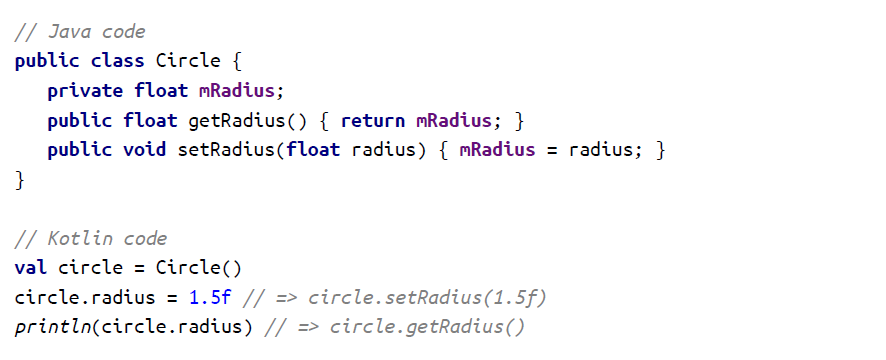
\includegraphics[scale=0.75]{Properties.png}
  \caption{{\bfseries Esempio di utilizzo delle proprietà}}
  \label{KotlinProperties}
\end{figure}

La figura \ref{KotlinProperties} rappresenta un esempio di come sia semplice la sintassi Kotlin per chiamare metodi getter e setter da classi definite in Java.\\

È inoltre possibile utilizzare questa sintassi delle proprietà di Kotlin per le classi definite in Java.\\
In particolare, getter in una classe Java sono accessibili come proprietà \texttt{val} da Kotlin, e le coppie getter/setter possono essere accedute come proprietà \texttt{var}. Ad esempio, se una classe Java definisce degli ipotetici metodi chiamati \texttt{getName()} e \texttt{setName()}, è possibile accedervi con una proprietà Kotlin denominata \texttt{name}. Se la classe Java definisce, ancora, dei metodi \texttt{isMarried()} e \texttt{setMarried()} per un ipotetico campo booleano, il nome della corrispondente proprietà Kotlin sarà \texttt{isMarried}; per cui, riprendendo l'esempio di classe generica \texttt{Person}, la sintassi delle proprietà sarà la seguente:\\

\begin{lstlisting}[caption={Utilizzo delle proprietà di una classe Kotlin}, captionpos=b, label={lst:exampleProperties}, language=Kotlin]
class Person(
  val name: String,
  var isMarried: Boolean
)

//Istanziazione

val bob = Person("Bob", true) //Oppure, in alternativa:
val bob = Person(name = "Bob", isMarried = true)  //In maniera piu' espressiva
val bob = Person(isMarried = true, name = "Bob")  //Ordine irrilevante con questa sintassi
\end{lstlisting}

Si noti, nell'esempio \ref{lst:exampleProperties}, come l'istanziazione di un oggetto nel linguaggio Kotlin non richieda l'utilizzo della keyword \texttt{new}. In Kotlin, è possibile, inoltre, definire dei valori di default da assegnare a proprietà della classe che si sta definendo, in modo da evitare la ripetizione non necessaria di codice che comporta, in Java, la scrittura di differenti costruttori per diversi set-up della classe, in cui vengono assegnati dei campi piuttosto che altri. Queste cosiddette "{\em default properties}" hanno la seguente sintassi:\\

\begin{lstlisting}[caption={Proprietà predefinite}, captionpos=b, label={lst:exampleDefProperties}, language=Kotlin]
class Person(val name: String, var isMarried: Boolean, val country: String = "Italy")

//Istanziazione

val bob = Person("Bob", true)
println(bob.country)          // Stampa "Italy"
\end{lstlisting}

Per quanto riguarda la definizione di Interfacce, il linguaggio Kotlin non differisce in maniera rilevante da Java: la keyword \texttt{interface} definisce un’interfaccia che ha le stesse peculiarità di una definita in Java, con la possibilità di definire implementazioni di default ai metodi (simile alle \texttt{abstract class} nel linguaggio Java) e default properties. Per dichiarare, nella definizione di una classe, la sua implementazione di una interfaccia, in Kotlin si utilizza la sintassi “\texttt{:}” per sostituire la keyword \texttt{implements} di Java (l'utilizzo dei due punti ha la stessa valenza nel creare gerarchie di classi: va quindi a sostituire anche la keyword \texttt{extends}).\\

\begin{lstlisting}[caption={Utilizzo della notazione "\texttt{:}"}, captionpos=b, label={lst:exampleEreditarietà}, language=Kotlin]
class Person(val name: String, var isMarried: Boolean) : Human  //implements
class Worker(val job: String) : Person                          //extends
\end{lstlisting}

Un ulteriore aspetto interessante riguarda le classi innestate, che non vengono considerate come "inner" di default: per specificarlo, è necessario aggiungere la keyword \texttt{inner} nella dichiarazione e incapsulare, così, il riferimento alla classe outer. Kotlin fornisce una ulteriore funzionalità: le classi \texttt{sealed} ("sigillate"); si contrassegna una superclasse con questo modificatore se si vuole limitare la possibilità di creare sue sottoclassi: tutte le sottoclassi dirette di una classe marcata come \texttt{sealed} devono, infatti, essere innestate nella loro superclasse.\\

\subsection{Data-Classes}
Con il termine data class si intende una classe che fornisca un supporto conveniente per immagazzinare e gestire dati; tipicamente, in Java, una data class deve implementare i metodi \texttt{toString}, \texttt{equals} e \texttt{hashCode}. Per quanto riguarda questa problematica, le IDE moderne permettono facilmente di generare automaticamente questi metodi e verificare che siano implementati correttamente e in modo coerente. In Kotlin viene fatto un passo ulteriore: non è più necessario esplicitare questi metodi. Questa funzionalità è messa a disposizione se si aggiunge il modificatore \texttt{data} alla classe, per fare in modo che vengano generati automaticamente ed implicitamente i metodi \texttt{toString}, \texttt{equals} e \texttt{hashCode}: questi verranno inferiti dal compilatore, permettendo di risparmiare decine di linee di codice. Si noti che le proprietà non dichiarate nel costruttore primario non prendono parte ai controlli di uguaglianza del metodo \texttt{equals} e al calcolo dell’\texttt{hashcode}.
Con questo particolare tipo di notazione, è possibile rendere il codice delle classi di questo tipo estremamente leggibile e snello: si noti, infatti, la perfetta equivalenza delle seguenti implementazioni di \texttt{data class}, la prima (esempio \ref{lst:exampleDataClassKt}) scritta in Kotlin, la seconda (esempio \ref{lst:exampleDataClassJava}) in Java.\\

\begin{lstlisting}[caption={Data Class in Kotlin}, captionpos=b, label={lst:exampleDataClassKt}, language=Kotlin]
data class Customer(val id: Long, val name: String)
\end{lstlisting}

\begin{lstlisting}[caption={Data Class corrispondente scritta in Java}, captionpos=b, label={lst:exampleDataClassJava}, language=Java]
public class Customer {
   	  private String id;
    	private String name;

      public Customer(String id, String name) {
        this.id = id;
        this.name = name;
    	}
    	public String getId() {
        return id;
    	}

    	public void setId(String id) {
        this.id = id;
    	}

   	  public String getName() {
        return name;
    	}

    	public void setName(String name) {
        this.name = name;
    	}

    	@Override
    	public boolean equals(Object o) {
        if (this == o) return true;
        if (o == null || getClass() != o.getClass()) return false;

        Customer customer = (Customer) o;

        if (id != null ? !id.equals(customer.id) : customer.id!=null) return false;
        return name != null ? name.equals(customer.name) customer.name == null;
    	}

    	@Override
   	  public int hashCode() {
        int result = id != null ? id.hashCode() : 0;
        result = 31 * result + (name != null ? name.hashCode() : 0);
        return result;
    	}
}
\end{lstlisting}

Le proprietà di una \texttt{data class} non devono necessariamente essere delle \texttt{val}, tuttavia, come già accennato, l’utilizzo di proprietà read-only è fortemente consigliato in Kotlin, per rendere le istanze di una \texttt{data class} immutabili. Gli oggetti immutabili possono risolvere molti problemi comuni, ad esempio, in parti di codice multithread: una volta creato, l’oggetto rimane nello stato originale e non è necessario preoccuparsi di altri thread che lo possano modificare durante l’esecuzione.\\
Per rendere ancora più semplice l'uso di istanze di data classes come oggetti immutabili, il compilatore Kotlin genera un ulteriore metodo che consente di copiare le istanze di queste classi, modificando, opzionalmente, i valori di alcune proprietà a scelta. Creare una copia è tipicamente una buona alternativa a modificare l'istanza in atto di una classe: la copia, infatti, ha un ciclo di vita separato e non può influenzare le aree del codice che si riferiscono all'istanza originale. È questa la funzione del metodo \texttt{copy()}, e si riporta di seguito un esempio del suo utilizzo:\\
\\

\begin{lstlisting}[caption={Utilizzo della funzione \texttt{copy}}, captionpos=b, label={lst:exampleCopy}, language=Kotlin]
val bob = Person("Bob", true)
println(bob.copy(isMarried = false)) // Stampa "Person(name="Bob", isMarried=false)"
\end{lstlisting}

\section{Cicli: operatori \texttt{when} e di range}

L’operatore \texttt{when} può essere pensato come corrispondente dello \texttt{switch} statement in Java, anche se incapsula alcune funzionalità che lo rendono più potente e molto più utilizzato e utilizzabile. Innanzitutto, come la struttura \texttt{if-else}, \texttt{when} è un'espressione che restituisce un valore: è possibile quindi scrivere una funzione con un expression body, restituendo direttamente l'espressione corrispondente al \texttt{when}.\\
Il codice trova il ramo corrispondente al valore della variabile passata in input all’operatore (a differenza di Java, non è necessario inserire istruzioni \texttt{break} in ogni ramo), se c’è un valore di un ramo che fa match con quello passato in input, solo quest’ultimo viene eseguito. A differenza dello \texttt{switch} statement, che richiede di utilizzare costanti (costanti \texttt{enum}, stringhe o numeri) come condizioni, con \texttt{when} è possibile utilizzare qualsiasi oggetto. Si noti nell'esempio successivo (\ref{lst:exampleWhen}) la definizione di una inline function che utilizza un \texttt{when} statement con due istanze della \texttt{enum class} \texttt{Color}:\\

\begin{lstlisting}[caption={Il costrutto \texttt{when}}, captionpos=b, label={lst:exampleWhen}, language=Kotlin]
fun mix(c1: Color, c2: Color) =
    when (setOf(c1, c2)) {          //setOf() e' una funzione di standard library
        setOf(RED, YELLOW) -> ORANGE
        setOf(YELLOW, BLUE) -> GREEN
        setOf(BLUE, VIOLET) -> INDIGO
        else -> throw Exception("Dirty color")
    }

/*...*/

println(mix(BLUE, YELLOW)) //Stampa "GREEN"
\end{lstlisting}

In questo esempio, se i colori \texttt{c1} e \texttt{c2} sono \texttt{RED} e \texttt{YELLOW} (o viceversa), il risultato della loro miscelazione è \texttt{ORANGE}, e così via, e per implementarlo, si utilizza il confronto fra \texttt{set}. La libreria standard di Kotlin contiene una funzione \texttt{setOf} (che si approfondirà nel paragrafo successivo) che crea un set contenente gli oggetti specificati come argomenti. Un set, come in Java, è una collezione per cui non è rilevante l'ordine degli oggetti contenuti, di conseguenza due set sono uguali se contengono gli stessi oggetti. Quindi, se i set \texttt{setOf(c1, c2)} e \texttt{setOf(RED, YELLOW)} sono uguali, significa che \texttt{c1} è \texttt{RED} e \texttt{c2} è \texttt{YELLOW}, o viceversa. La funzione \texttt{setOf(c1, c2)} viene controllata per uguaglianza: prima con \texttt{setOf(RED, YELLOW)} e poi con gli altri set di colori corrispondenti ai vari rami dell’espressione \texttt{when}, uno dopo l'altro. Se nessuna delle condizioni degli altri rami risulta soddisfatta, viene valutato il ramo \texttt{else}.\\
Essere in grado di utilizzare qualsiasi espressione come una condizione di un ramo di espressione \texttt{when} consente, in molti casi, di scrivere codice elegante e conciso.\\
Le operazioni di iterazione in Kotlin sono particolarmente simili a quelle corrispondenti nel linguaggio Java: i cicli \texttt{while} e \texttt{do-while} risultano perfettamente identici a quelli di Java, mentre il for loop esiste in un’unica forma, che è equivalente al ciclo \texttt{for-each} di Java e viene scritto come \texttt{for <item> in <elements>}, con la stessa sintassi presente in C\#.\\
Come è stato appena menzionato, in Kotlin non c'è il for loop classico di Java, dove si inizializza un variabile, se ne aggiorna il valore ad ogni iterazione e si chiude il ciclo quando il valore raggiunge un certo limite. Per sostituire i casi d’uso più comuni di tali cicli, Kotlin utilizza il concetto di {\em range}. Un range è essenzialmente un semplice intervallo tra due valori, di solito numeri, e viene rappresentato con l’operatore "\texttt{..}":\\

\begin{lstlisting}[caption={Utilizzo dell'operatore di range}, captionpos=b, label={lst:exampleRange}, language=Kotlin]
val oneToTen = 1..10
\end{lstlisting}

Si noti che gli intervalli in Kotlin sono chiusi o inclusivi, il che significa anche il secondo valore (il limite superiore del range) risulta sempre parte della gamma. Questi costrutti, espressi su valori interi, possono essere utilizzati, appunto, in maniera elementare per eseguire dei loop su tutti i valori del range: in questo caso tale intervallo è chiamato "{\em progression}". È possibile utilizzare l'operatore \texttt{in} in espressioni condizionali per verificare l’appartenenza di un valore ad un intervallo, oppure il suo opposto (\texttt{!in}) per verificarne la non-appartenenza.\\
Oltre che con valori interi, i range possono essere utilizzati anche per i \texttt{character}, ma non solo: con una qualsiasi classe che supporta il confronto fra istanze (implementando l'interfaccia \texttt{java.lang.Comparable}) è possibile creare dei range di istanze di tale classe. Si riporta di seguito un esempio dell'utilizzo dell'operatore di range all'interno di un'espressione \texttt{when}:\\
\\

\begin{lstlisting}[caption={Operatore di range con valori interi all'interno di una espressione \texttt{when}}, captionpos=b, label={lst:exampleRangeWhen}, language=Kotlin]
val myInt = 12
val x = when (myInt) {
    0 -> "zero"
    1, 2 -> "one or two"
    in 3..10 -> "small number"
    in 11..Int.MAX_VALUE -> "large number"
    else -> "negative number"
}
println(x)    //Stampa "large number"
\end{lstlisting}

\section{Collections ed Infix Calls}
Come già espresso nel capitolo precedente, la forte interoperabilità con Java da parte del linguaggio sviluppato da JetBrains può essere riscontrata anche dal fatto che Kotlin utilizza le classi del Java Collection Framework: non dispone, infatti, di un proprio set di classi di collezione. Questa scelta è dovuta al fatto che usare le collezioni standard di Java rende, appunto, molto più semplice e immediato interagire con il codice Java: non è necessario convertire le collezioni in alcun modo quando si utilizzano funzioni Java da codice Kotlin o viceversa. Tuttavia, gli sviluppatori del team Kotlin hanno aggiunto ulteriori funzionalità al già esteso Collection Framework di Java, permettendo di semplificare diverse operazioni, come ad esempio, ottenere l'ultimo elemento di un elenco (funzione di libreria \texttt{last}) o trovare un massimo in una collection di numeri (funzione di libreria \texttt{max}), oltre che delle funzioni utili per dichiarare in maniera più intuitiva ed immediata alcune collezioni: oltre alla precedentemente discussa funzione \texttt{setOf} per creare un \texttt{Set} di oggetti; esistono altre due funzioni molto simili, utilizzate per generare Liste e Mappe.\\

\begin{lstlisting}[caption={Funzioni di libreria per le collezioni}, captionpos=b, label={lst:exampleCollections}, language=Kotlin]
val set = setOf(1, 7, 53)
val list = listOf(1, 7, 53)
val map = mapOf(1 to "one", 7 to "seven", 53 to "fifty-three")
\end{lstlisting}

Si noti che, nella terza funzione, l’operatore "\texttt{to}" non è un costrutto speciale, ma una normale funzione: si tratta di un particolare tipo di invocazione, chiamata {\em infix call}. In questo particolare tipo di chiamata, il nome del metodo viene posto tra il nome dell'oggetto di destinazione e quello del parametro di input, senza separatori aggiuntivi, rendendo l’invocazione della funzione molto più leggibile e simile ad un linguaggio "human-like". In Kotlin, dunque, le seguenti due chiamate risultano equivalenti:\\

\begin{lstlisting}[caption={La sintassi di una infix call}, captionpos=b, label={lst:exampleInfix}, language=Kotlin]
1.to("one") //  Chiamata con sintassi standard
1 to "one"  //  Chiamata con infix call
\end{lstlisting}

L'elevata potenzilalità delle chiamate infix sta nel fatto che possono essere utilizzate con qualsiasi metodo che richieda un singolo parametro in ingresso: per consentire la chiamata a una funzione utilizzando la notazione infix, è necessario contrassegnarlo con il modificatore \texttt{infix}. Nel seguente esempio (\ref{lst:exampleInfixTo}) si può notare una versione semplificata della dichiarazione della funzione \texttt{to}:\\

\begin{lstlisting}[caption={Definizione della funzione \texttt{to}}, captionpos=b, label={lst:exampleInfixTo}, language=Kotlin]
infix fun Any.to(other: Any) = Pair(this, other)
\end{lstlisting}

Essa restituisce un'istanza di \texttt{Pair}, una classe della Kotlin standard library che rappresenta una coppia di elementi (in questa libreria è presente anche la classe per rappresentare una tripla di elementi, ovvero \texttt{Triple}). Un altro esempio di utilizzo di questo costrutto, è l'assegnazione di una coppia di elementi direttamente a due variabili distinte utilizzando una singola linea di codice:\\

\begin{lstlisting}[caption={Infix call e destructured declaration}, captionpos=b, label={lst:exampleDestructured}, language=Kotlin]
val (number, name) = 1 to "one"

println(number)   //Stampa "1"
println(name)     //Stampa "one"
\end{lstlisting}

Questa caratteristica è chiamata "dichiarazione destrutturata" e non è limitata alle istanze di classe \texttt{Pair}: è possibile utilizzarla, ad esempio, per assegnare una entry di una mappa a due variabili separate, chiave e valore. Dall'esempio \ref{lst:exampleInfixTo}, in cui si definisce la funzione \texttt{to}, si può facilmente notare la particolarità della sua dichiarazione: questa funzione, infatti, appartiene ad una particolare famiglia: le cosiddette {\bfseries Extension Functions} di Kotlin.\\

\section{Extension Functions ed Extension Properties}
Una delle funzionalità principali di Kotlin, che risponde perfettamente alla filosofia del linguaggio di richiedere una massima integrazione con il codice esistente, sono le Extension Functions. Anche i progetti Kotlin "puri" sono costruiti sopra a librerie Java come il JDK, il framework Android, e/o altri framework di terze parti, ma in particolare nei progetti cosiddetti "ibridi", quando si integra Kotlin in un progetto Java, ci si trova a dover utilizzare anche del codice esistente che non è stato o non verrà convertito in Kotlin. Le funzioni di estensione ({\bfseries Extension Functions}) consentono di utilizzare il linguaggio Kotlin sopra a quello Java, in maniera del tutto trasparente e senza doverlo riscrivere. Concettualmente, una Extension Function è una funzione che può essere chiamata come membro di una certa classe ma è definita al di fuori di essa; nel seguente esempio, si aggiungerà alla classe \texttt{String} un metodo per calcolare l’ultimo carattere di una stringa:\\
\begin{lstlisting}[caption={Definizione di una Extension Function}, captionpos=b, label={lst:exampleExtrnsionF}, language=Kotlin]
fun String.lastChar(): Char = this.get(this.length - 1)
\end{lstlisting}

Come si può notare, tutto ciò che richiede la sintassi delle Extension Functions è inserire il nome della classe o dell'interfaccia che si intende estendere prima del nome della funzione che si sta aggiungendo (separandoli con un punto). Il nome della classe che si vuole estendere è denominato "{\em receiver type}", mentre il valore su cui si sta chiamando la funzione di estensione è chiamato "{\em receiver object}" (nell'esempio \ref{lst:exampleExtrnsionF} si tratta del riferimento a "\texttt{this}"). Una volta definita, è possibile chiamare la funzione di estensione usando la stessa sintassi utilizzata per i membri ordinari della classe:\\

\begin{lstlisting}[caption={Chiamata di una Extension Function}, captionpos=b, label={lst:exampleExtensionFCalling}, language=Kotlin]
println ("Hello, Kotlin".lastChar())  //Stampa "n"
\end{lstlisting}

La chiamata riportata in nell'esempio \ref{lst:exampleExtensionFCalling}, in cui \texttt{String} è receiver type mentre la stringa \texttt{"Hello, Kotlin"} è il receiver object, stamperà sullo standard output una stringa contenente la sola lettera "n". In questo modo, si è aggiunto un metodo personalizzato alla classe \texttt{String}, senza che essa facesse parte del codice. Non è rilevante, inoltre, che la classe da cui si intende estendere una funzione sia scritta in Java, Kotlin o in un altro linguaggio JVM, come Groovy: fintanto che è compilata in un file Java \texttt{.class}, è possibile aggiungervi le proprie estensioni.\\
Quando si definisce una funzione di estensione, essa non viene resa automaticamente disponibile all'interno dell'intero progetto, deve, invece, essere opportunamente importata, proprio come qualsiasi altra classe o funzione; ciò aiuta ad evitare accidentali conflitti di nomi. L’importazione avviene utilizzando la stessa sintassi utilizzata per le classi, con la possibilità di cambiare il nome della classe o della funzione che si sta importando utilizzando la parola chiave "\texttt{as}": questo può risultare molto utile quando si dispone di diverse funzioni con lo stesso nome in diversi package e si desidera utilizzarle nello stesso file.
Nel corpo di una funzione di estensione, si usa \texttt{this} allo stesso modo in cui si utilizza in un metodo (quindi i riferimenti \texttt{this} possono essere anche, ad esempio, omessi); è possibile, inoltre, accedere direttamente ai metodi e alle proprietà della classe che si sta estendendo, come se si stesse scrivendo una funzione nella classe stessa. Tuttavia, un limite sta nel fatto che le funzioni di estensione non consentono di violare l'incapsulamento: a differenza dei metodi definiti nella classe, le Extension Functions non hanno accesso a membri privati o protetti della classe.\\

Chiamare una Extension Function non comporta la creazione di oggetti adapter o di qualsiasi altro overhead di runtime: una funzione di estensione è, infatti, semplicemente un metodo statico che accetta il receiver object come suo primo argomento. Questo rende il loro utilizzo piuttosto semplice anche in Java: chiamando il metodo statico e passando l'istanza dell'oggetto ricevente. Proprio come per altre funzioni top-level, il nome della classe Java contenente il metodo viene determinato dal nome del file dove viene dichiarata la funzione.\\
Poiché le funzioni di estensione sono effettivamente solo zucchero sintattico sulle chiamate ad un metodo statico, è possibile utilizzare un tipo più specifico come receiver type, non per forza una semplice classe. Se, per esempio, si vuole creare una funzione \texttt{join} che possa essere invocata solo su Collections di stringhe, allora chiamare questa funzione passandovi una lista di oggetti di un altro tipo non dovrebbe funzionare. Inoltre, la natura statica delle funzioni di estensione non permette che vengano sovrascritte nelle sottoclassi.\\
Si noti, infine, che se una classe ha una funzione membro con la stessa signature di una funzione di estensione, la funzione membro ha sempre la precedenza.\\

Le {\bfseries Extension Properties} forniscono un ulteriore modo per estendere le classi con API accessibili utilizzando la sintassi delle proprietà, piuttosto che la sintassi delle funzioni. Anche se sono chiamate "proprietà", esse non possono avere alcuno stato: non è possibile aggiungere ulteriori campi ad istanze esistenti di oggetti Java. Nell'esempio \ref{lst:exampleExtrnsionF} è stata definita una funzione lastChar: nel seguente snippet, verrà convertita in proprietà:\\

\begin{lstlisting}[caption={Definizione di una Extension Property}, captionpos=b, label={lst:exampleExtensionP}, language=Kotlin]
val String.lastChar: Char get() = get(length - 1)
\end{lstlisting}

Come si può notare dall'esempio \ref{lst:exampleExtensionP}, come per le funzioni, una proprietà di estensione si definisce sintatticamente come una normale proprietà, aggiungendo un receiver type. Il getter, inoltre, deve sempre essere definito, poiché non è presente nessun campo di backup per la proprietà, e quindi nessuna implementazione di getter standard; per la stessa ragione, gli inizializzatori non sono consentiti: non vi è un campo dove memorizzare il valore specificato come initializer. Se la classe da cui si intende estendere è, invece, modificabile, è consentito definire anche un setter.\\
L'accesso alle proprietà di estensione viene effettuato esattamente allo stesso modo delle member properties: quando è necessario accedere a una proprietà di estensione da Java, è necessario invocare il suo getter in modo esplicito, come avviene per le normali proprietà Kotlin.\\

\section{Null Safety}
Un'altra delle funzionalità più importanti e più innovative del linguaggio Kotlin è la cosiddetta {\em Nullability}.\\
La nullabilità è una caratteristica del type system di Kotlin che aiuta ad evitare e controllare le occorrenze di \texttt{NullPointerException}: l'approccio dei moderni linguaggi, incluso Kotlin, è quello di convertire questi problemi da errori di runtime a errori di compilazione. Sostenendo la nullabilità come parte del type system, il compilatore può rilevare molti errori possibili durante la compilazione e ridurre la possibilità di avere eccezioni tirate a runtime. La prima, e probabilmente più importante, differenza tra il type system di Kotlin e quello di Java è il sostegno esplicito di Kotlin per i tipi di nullable. Questo significa che Kotlin fornisce un modo per indicare quali variabili o proprietà all'interno di un programma possono essere \texttt{null}: concettualmente, se un la variabile può essere \texttt{null}, chiamare un metodo su di essa non è sicuro, poiché può portare ad una \texttt{NullPointerException}. Per vedere come funziona in pratica, si consideri la seguente funzione Java:\\

\begin{lstlisting}[caption={Funzione \texttt{strLen} definita in Java}, captionpos=b, label={lst:exampleNullJava}, language=Java]
/* Java */

int strLen(String s) {
  return s.length();
}
\end{lstlisting}
Non si tratta di una funzione sicura, in quanto, se chiamata con un argomento con valore \texttt{null}, causerà una \texttt{NullPointerException}. Per evitare questo tipo di errore, in Java, è necessario aggiungere un controllo al momento della chiamata della funzione. Traducendo questa dichiarazione in Kotlin, è possibile pensarla chiedendosi se si prevede che la funzione sia chiamata con un argomento nullo, oppure no. Se non si prevede che ciò accada, questa funzione si dichiara in Kotlin come segue:\\

\begin{lstlisting}[caption={Funzione Kotlin che non accetta \texttt{null} come argomento}, captionpos=b, label={lst:exampleNullKt}, language=Kotlin]
fun strLen(s: String) = s.length
\end{lstlisting}

Dunque, nell'ambiente Kotlin, chiamare \texttt{strLen} (così come viene definita nell'esempio \ref{lst:exampleNullKt}) con un argomento che può essere nullo non è consentito e verrà segnalato come errore al momento della compilazione. Il parametro viene dichiarato come tipo \texttt{String}, e in Kotlin questo significa che deve sempre contenere un'istanza di \texttt{String}: è un’imposizione del compilatore, quindi non è possibile passare un argomento contenente \texttt{null}, con la garanzia che la funzione \texttt{strLen} non lancerà mai un \texttt{NullPointerException} durante il runtime. Se, d'altra parte, si desidera consentire l'utilizzo di questa funzione con tutti gli argomenti, inclusi quelli che potrebbero essere \texttt{null}, è necessario contrassegnarlo esplicitamente inserendo un punto interrogativo dopo il nome del tipo dell'argomento:\\

\begin{lstlisting}[caption={Funzione Kotlin null-safe}, captionpos=b, label={lst:exampleNull?Kt}, language=Kotlin]
fun strLenSafe(s: String?) = /*...*/
\end{lstlisting}

È possibile usare questa notazione (come nell'esempio \ref{lst:exampleNull?Kt}) inserendo il punto interrogativo dopo qualsiasi tipo, per indicare che i valori di questo tipo possono memorizzare riferimenti \texttt{null}: \texttt{String?}, \texttt{Int?}, \texttt{Person?},\texttt{MyCustomType?}, e così via. Avendo introdotto questa particolare notazione, dunque, un tipo espresso senza un punto interrogativo indica che le variabili di questo tipo non possono memorizzare riferimenti \texttt{null}. Ciò significa che tutti i tipi normali sono di default non-null, a meno che non esplicitamente contrassegnati come nullable; si noti che, a tempo di esecuzione, oggetti di tipo \texttt{null} o non-null sono gli stessi: un tipo nullable non è un wrapper per un tipo non-nullo. Tutti i controlli vengono eseguiti a tempo di compilazione e ciò significa che non si aggiunge alcun overhead di runtime nel lavorare con i tipi nullable. Una volta che si dispone di un valore di tipo nullable, l'insieme di operazioni che è possibile eseguire su di esso è limitato: ad esempio, non è più possibile chiamare metodi su di esso, né assegnarlo a una variabile di tipo non nullo e né passarlo come parametro a una funzione che prevede un argomento non nullo:\\

\begin{lstlisting}[caption={Alcuni utilizzi delle funzioni definite in precedenza}, captionpos=b, label={lst:exampleNullKtVari}, language=Kotlin]
fun strLenSafe(s: String?) = s.length   //ERRORE a tempo di compilazione
fun strLenSafe(s: String?) = s?.length  //OK

val x: String? = null  //OK
var y: String = x      //ERRORE a tempo di compilazione
var y: String? = x     //OK

strLen(x)     //ERRORE a tempo di compilazione
strLenSafe(x) //OK
\end{lstlisting}

Per poter utilizzare un valore nullable, è necessario confrontarlo precedentemente con \texttt{null} e, una volta eseguito il confronto, il compilatore tratterà il valore come non-null nello scope dove il controllo è stato eseguito. Di seguito si riporta un esempio con del codice perfettamente valido:\\

\begin{lstlisting}[caption={Aggirare i valori \texttt{null} grazie alla nullability}, captionpos=b, label={lst:exampleNullKtElse}, language=Kotlin]
fun strLenSafe(s: String?): Int = if (s != null) s.length else 0

val x: String? = null
println(strLenSafe(x))     // Stampa "0"
println(strLenSafe("abc")) // Stampa "3"
\end{lstlisting}

Fortunatamente, Kotlin fornisce una serie di altre funzionalità per aiutare a gestire i valori nullable in modo più conciso ed elegante:\\

\subsection{Operatore di chiamata sicura {\bfseries \texttt{?.}}}
Il {\em safe call operator} è considerato uno degli strumenti più utili nell'arsenale di Kotlin e si utilizza semplicemente, aggiungendo il punto interrogativo immediatamente prima del punto, nella chiamata ad una funzione. Esso permette di combinare un controllo di null safety e una chiamata di metodo in un'unica operazione. In altre parole, se il valore su cui si sta tentando di chiamare il metodo non è nullo, la chiamata di metodo viene eseguita normalmente; se invece è null, la chiamata viene {\bfseries ignorata} e viene utilizzato \texttt{null} come valore. Si noti che il tipo di risultato di tale invocazione è nullable. È possibile utilizzare l'operatore di safe call anche per accedere alle proprietà, non solo per le chiamate di metodo.\\

\begin{lstlisting}[caption={Utilizzo di safe call operator}, captionpos=b, label={lst:exampleSafeCall}, language=Kotlin]
fun strLenSafe(s: String?) = s?.length
\end{lstlisting}

\subsection{Elvis operator {\bfseries \texttt{?:}}}
Questo operatore (anche noto come "{\em null-coalescing operator}") è utile per fornire valori predefiniti al posto di \texttt{null}:\\

\begin{lstlisting}[caption={Utilizzo di null-coalescing operator}, captionpos=b, label={lst:exampleNullCoalescing}, language=Kotlin]
fun strLenSafe(s: String?):Int = s?.length ?: 0
\end{lstlisting}
Questa notazione permette di semplificare la deinizione di funzione dell'esempio \ref{lst:exampleNullKtElse} e  sta a significare che se la stringa \texttt{s} è \texttt{null}, la funzione restituirà 0 come valore di lunghezza. L'operatore prende dunque due valori e il suo risultato è il primo, se non è nullo, altrimenti si assegna il secondo. L'operatore Elvis viene spesso utilizzato insieme all'operatore di chiamata sicura (come nell'esempio) per sostituire un valore diverso da \texttt{null} quando l'oggetto su cui viene chiamato il metodo è nullo. Ciò che rende l'operatore Elvis particolarmente utile in Kotlin è il fatto che operazioni come \texttt{return} e \texttt{throw} lavorano come espressioni e quindi possono essere utilizzati come secondo valore dell'operatore: in questi casi, se il valore sul lato sinistro è null, la funzione restituirà immediatamente un valore o lancerà un'eccezione.\\

\subsection{Cast sicuri con {\bfseries \texttt{as?}}}
Proprio come un normale type cast di Java, l’operatore \texttt{as} lancia una \texttt{ClassCastException} se il valore non possiede il tipo di cui si sta cercando di fare il cast; per evitare questo problema, in Java, è possibile combinare l’operazione con un controllo \texttt{is} o {\texttt{istanceof} per assicurarsi che l’eccezione non venga lanciata. In Kotlin, invece, viene proposta un'alternativa più sicura e concisa: il safe cast operator "\texttt{as?}": esso tenta di eseguire il cast di un valore al tipo specificato e restituisce \texttt{null} se il valore non possiede il tipo appropriato.\\

\begin{lstlisting}[caption={Utilizzo di safe casting}, captionpos=b, label={lst:exampleSafeCast}, language=Kotlin]
val y = null
val x: String? = y as? String //x ha valore null, nessun errore
\end{lstlisting}

\subsection{Asserzioni di not-null {\bfseries \texttt{!!}}}
Gli operatori di safe call, safe cast e null-coalescing risultano molto utili e appaiono spesso in un normale programma Kotlin; tuttavia, a volte può essere necessario specificare che un valore che si sta utilizzando è effettivamente ed esplicitamente non-nullo. L'asserzione di not-null è lo strumento più semplice che Kotlin mette a disposizione per lavorare con valori di tipo nullable: è rappresentato da un doppio punto esclamativo e converte, appunto, qualsiasi valore a un tipo non nullo. Se si usa l’asserzione di not-null su un valore che, a un certo punto del codice, potrebbe risultare nullo, Kotlin lancerà una \texttt{NullPointerException} {\bfseries a runtime}; per questo motivo, questo operatore va usato con parsimonia all’interno di un progetto, ed esclusivamente su valori su cui è assolutamente assicurata la non-nullabilità. Ci possono essere, infatti, situazioni in cui le asserzioni non-null sono la soluzione appropriata per un problema: ad esempio, quando si esegue un null check in una funzione e si utilizza il valore in un'altra funzione, il compilatore non può inferire che esso sia "sicuro"; dunque, se ci si è assicurati che il controllo è sempre eseguito in un'altra funzione e non si desidera duplicarlo prima di utilizzare il valore, è possibile (e consigliato) utilizzare un'asserzione di not-null.\\

Nella figura \ref{NullSafety} vengono riportati alcuni esempi di chiamate a variabili custom attraverso operatori di null-safety e non, confrontando il linguaggio Kotlin con Java.\\

\begin{figure}[ht]
  \centering
  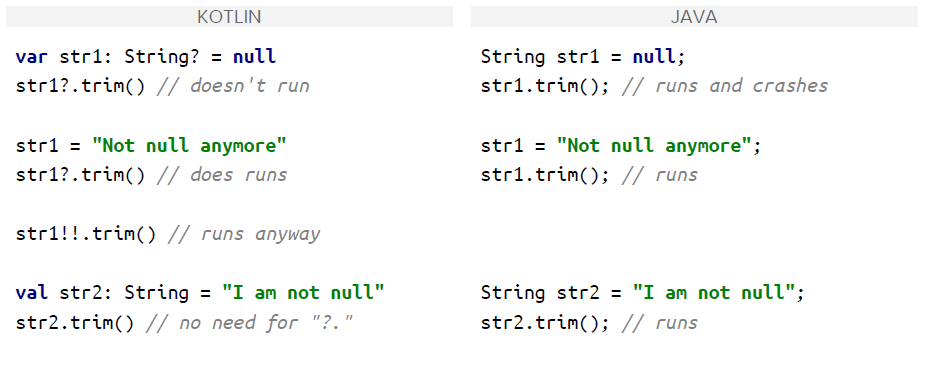
\includegraphics[scale=0.66]{NullSafety.png}
  \caption{{\bfseries Esempio generico degli operatori di Null-Safety}}
  \label{NullSafety}
\end{figure}

    %% Direttive TeXworks:
% !TeX root = ../semprini_luca_tesi.tex
% !TEX encoding = UTF-8 Unicode
% !TEX program = arara
% !TEX TS-program = arara
% !TeX spellcheck = it-IT

%% Direttive Arara:
% arara: pdflatex: { shell: yes, synctex: yes, action: batchmode, options: "-halt-on-error -file-line-error-style" }
% arara: frontespizio
% arara: biber
% arara: pdflatex: { shell: yes, synctex: yes, action: batchmode, options: "-halt-on-error -file-line-error-style" }
% arara: pdflatex: { shell: yes, synctex: yes, action: nonstopmode, options: "-halt-on-error -file-line-error-style" }
\chapter{Kotlin in Android}
Lo scopo primario dello sviluppo di Kotlin da parte di JetBrains non era, inizialmente, quello di trovare un nuovo linguaggio per sviluppare progetti Android. Tuttavia, appoggiandosi sulla JVM, fin dalla prima release sono state messe a fuoco le sue grandi potenzialità per costruire applicazioni su questa piattaforma. Con il passare dei mesi, questo contesto è divenuto il più popolare ed il più apprezzato dagli estimatori di Kotlin, tanto da portare, in via del tutto prematura e potenzialmente rischiosa, molte software house (ma anche sviluppatori indipendenti) a puntare su questo linguaggio per lo sviluppo delle proprie applicazioni mobile. Questa scommessa viene ripagata il 17 maggio 2017, data in cui il supporto ufficiale di Kotlin per questa piattaforma viene annunciato al Google I / O: da questa conferenza la popolarità del linguaggio di JetBrains cresce a dismisura ed il numero di progetti sviluppati interamente ed esclusivamente in Kotlin aumenta in maniera esponenziale.\\

\section{Perché Kotlin su Android?}
Il team di Android afferma di aver operato la scelta di rendere Kotlin un linguaggio ufficialmente supportato in quanto ritiene che sia "brillantemente progettato e maturo e renderà lo sviluppo di Android più veloce e divertente"; era già stato inoltre adottato, come accennato, da alcuni importanti sviluppatori (come Expedia, Flipboard, Pinterest, Square e altri) per le loro applicazioni di produzione. Un’altra discriminante nella scelta del supporto ufficiale è stata, ovviamente, "l'interoperabilità senza sforzo2 con Java: i programmatori Android che utilizzano tradizionalmente Java non avranno alcune difficoltà nell’apprendere la sintassi e la filosofia di Kotlin e sarà per essi molto più semplice iniziare ad utilizzare sempre più il nuovo linguaggio di JetBrains nelle loro applicazioni. Inoltre, essendo un linguaggio sviluppato dalla medesima compagnia produttrice di IntelliJ IDEA (sulla quale, tra le altre cose, è basata la stessa IDE ufficiale di Google Android Studio), non sorprende che il supporto IDE per Kotlin sia certamente eccellente per un linguaggio così giovane: mentre nelle versioni precedenti dell’IDE, il supporto a Kotlin era garantito esclusivamente installando un opportuno plug-in, a partire da Android Studio 3.0, Kotlin diventa un linguaggio di programmazione totalmente supportato su Android, venendo completamente incorporato come linguaggio principale e lascia all’utente scegliere se compilare in un bytecode compatibile con Java 6 o con Java 8.\\

Le funzionalità linguistiche di Kotlin, combinate con un plug-in di compilazione che supporta il framework Android, possono trasformare lo sviluppo di applicazioni per questa piattaforma in un'esperienza molto più produttiva e piacevole. Pattern di programmazione molto comuni nello sviluppo, ad esempio l'aggiunta di \texttt{Listener} ai controlli o il binding degli elementi di layout ai campi, possono essere compiuti utilizzando molte meno linee di codice, o addirittura, a volte, senza bisogno di scrivere codice: il compilatore, infatti, può generare automaticamente parti consistenti di questi controlli. Un altro grande vantaggio di utilizzare Kotlin è la migliore affidabilità a livello di applicazione: spesso, infatti ci si imbatte in errori che portano al crash dell’intera applicazione, come un'eccezione non gestita (spesso, una \texttt{NullPointerException}); il sistema di tipi di Kotlin, con il suo preciso monitoraggio dei valori \texttt{null}, rende questo comune problema molto meno pressante. La maggior parte del codice che in Java avrebbe portato a una \texttt{NullPointerException}, non riesce a compilare in Kotlin, il che assicura di poter individuare l'errore a tempo di compilazione, quindi evitando crash inaspettati durante l’esecuzione. Allo stesso tempo, poiché Kotlin è completamente compatibile anche con Java 6, il suo utilizzo non introduce nessun tipo di preoccupazione a livello di compatibilità di codice. Un ulteriore vantaggio è rappresentato dall’utilizzo delle espressioni lambda: molte delle funzioni di standard library di Kotlin consentono di sintetizzarle in un’unica linea, rendendo il codice più compatto ed intuitivo.\\

\section{Funzionalità utili per lo sviluppo Android}
Sono state accennate nel paragrafo precedente alcune caratteristiche e pattern di programmazione incorporati da Kotlin che possono rendere lo sviluppo di applicazioni Android più intuitivo ed elegante. Di seguito saranno analizzati i più significativi.\\

\subsection{Lambda Expressions}
Le {\em Lambda Expressions}, o semplicemente lambda, sono essenzialmente frammenti di codice che possono essere passati ad altre funzioni e la loro introduzione in Java 8 è stato uno dei cambiamenti più attesi nell'evoluzione del principale linguaggio JVM. La standard library di Kotlin ne fa uso in maniera ampia e con esse è possibile estrarre facilmente strutture di codice comuni rendendole funzioni di libreria: le lambda possono essere utilizzate anche con le librerie Java, a conferma della piena interoperabilità tra i due linguaggi, anche con quelle che non sono state originariamente concepite per supportare espressioni lambda. Uno degli usi più comuni per questi particolari costrutti è utilizzarli per lavorare con le collezioni, o all'interno di listeners, nello specifico ambiente Android.\\

Passare e memorizzare pezzi di comportamento nel codice è un compito frequente quando si tratta di lavorare con progetti complessi: questo tipo di problema è affrontato principalmente dalla programmazione funzionale, che offre un approccio differente da quello della programmazione Object-Oriented per risolvere questa questione; essa offre, infatti, la capacità di trattare le funzioni come valori. Invece di dichiarare una classe e di passarne un'istanza ad un metodo, è possibile passare direttamente una funzione, rendendo il codice è ancora più conciso. Non è necessario, inoltre, dichiarare esplicitamente una funzione, ma si può decidere di passare un blocco di codice direttamente come parametro di metodo. Di seguito si riporta nell'esempio \ref{lst:exAmpleLambda} una definizione di un Listener responsabile della gestione di click in Java 7. Questo ascoltatore implementa la corrispondente interfaccia \texttt{OnClickListener} con un metodo, \texttt{onClick}:\\

\begin{lstlisting}[caption={Definizione di \texttt{OnClickListener} in Java}, captionpos=b, label={lst:exAmpleLambda}, language=Java]
button.setOnClickListener(new OnClickListener() {
  @Override
  public void onClick(View view) {
      /* actions on click */
  }
});
\end{lstlisting}

Si noti la verbosità eccessiva, necessaria per dichiarare una classe interna anonima per esprimere il comportamento di un bottone nel momento in cui viene cliccato: questo pattern, se ripetuto molte volte, aumenta la complessità e intacca la leggibilità di un programma. In Kotlin, come in Java 8, è possibile utilizzare una lambda per questo comportamento:\\

\begin{lstlisting}[caption={Definizione di una lambda in Kotlin}, captionpos=b, label={lst:exAmpleLambdaConciso}, language=Kotlin]
button.setOnClickListener { view -> /* ... actions on click */ }
\end{lstlisting}

Lo snippet di codice nell'esempio \ref{lst:exAmpleLambdaConciso} Kotlin opera allo stesso modo di una classe anonima in Java (come nell'esempio \ref{lst:exAmpleLambda}) ma risulta molto più conciso e leggibile.\\
Un classico uso delle espressioni lambda è effettuato nel contesto delle Collezioni: la maggior parte delle attività che coinvolgono il Collection framework, infatti, seguono alcuni pattern comuni, quindi il codice che li implementa dovrebbe essere standardizzato in una qualche libreria; tuttavia questo risulta difficile senza fare uso di lambda.\\
Un classico esempio di come Kotlin integra all'interno della sua standard library delle funzioni che permettono, attraverso l'uso delle lambda, di semplificare il lavoro con le collezioni è la funzione \texttt{maxBy}, che permette di trovare il massimo elemento di una qualsiasi collezione, specificando quali valori debbano essere confrontati per trovarlo, appunto attraverso una lambda expression:\\

\begin{lstlisting}[caption={La funzione \texttt{maxBy}}, captionpos=b, label={lst:exAmpleLambdamaxBy}, language=Kotlin]
val people = listOf(Person("Frank", 29), Person("Bob", 31))
people.maxBy({ p: Person -> p.age })  // Stampa "Person(name=Bob, age=31)"
\end{lstlisting}

Nell'esempio \ref{lst:exAmpleLambdamaxBy} si suppone di aver definito una semplice classe \texttt{Person}, che prenda come parametri il nome di battesimo e l'età di una persona, quindi leggermente differente da quella definita nel capitolo precedente. La funzione \texttt{maxBy}, in questo specifico caso, è chiamata per trovare la persona più anziana all’interno della lista \texttt{people}, senza fare uso esplicito di cicli: il codice tra le parentesi graffe \texttt{{ p: Person -> p.age }} è una lambda che attua questa specifica logica. La funzione riceve un oggetto \texttt{Person} della lista come argomento (referenziato dalla variabile "\texttt{p}") e restituisce un valore da confrontare, in questo caso specifico si tratta dell'età, immagazzinata nella proprietà "\texttt{age}". Tuttavia questo codice risulta ancora alquanto verboso: in primo luogo, vi è ancora troppa punteggiatura, che danneggia la leggibilità, inoltre il tipo \texttt{Person} può essere dedotto dal contesto da parte del compilatore e quindi può essere omesso; infine, in Kotlin, non è necessario assegnare un nome all'argomento che prende in ingresso la lambda in questo caso.\\
Di seguito, verranno forniti esempi in cui si eseguiranno miglioramenti graduali alla sintassi, fino ad arrivare ad una forma espressiva ideale e che rispetti appieno la filosofia di Kotlin. Come prima cosa si rimuoveranno le parentesi: una convenzione sintattica consente di spostare una espressione lambda dalle parentesi tonde se essa è l'ultimo argomento in una chiamata di funzione. In questo esempio specifico (\ref{lst:exAmpleLambdamaxByNoPar}), tuttavia, la lambda expression è l'unico argomento, quindi è anche possibile rimuovere completamente le parentesi tonde dalla chiamata:\\

\begin{lstlisting}[caption={Rimozione delle parentesi tonde}, captionpos=b, label={lst:exAmpleLambdamaxByNoPar}, language=Kotlin]
people.maxBy { p: Person -> p.age }
\end{lstlisting}

Queste differenti forme sintattiche hanno esattamente la stessa semantica, con la differenza che l'ultima risulta essere la più semplice da leggere. Nel caso in cui si voglia passare due o più lambda, non è possibile muoverne più di una, quindi è tipicamente consigliabile passarle utilizzando la sintassi regolare.\
Procedendo con la semplificazione della sintassi, come accennato precedentemente, si può facilmente notare che si può fare a meno di specificare il tipo del parametro che la lambda prende in ingresso, in quanto il compilatore di Kotlin riuscirà a dedurlo dal contesto:\\

\begin{lstlisting}[caption={Rimozione della specificazione di tipo dalla lambda}, captionpos=b, label={lst:exAmpleLambdamaxByNoType}, language=Kotlin]
people.maxBy { p -> p.age }
\end{lstlisting}

Con la funzione \texttt{maxBy}, in particolare, il tipo del parametro è sempre uguale al tipo dell'elemento della collezione: siccome in questo caso si sta chiamando \texttt{maxBy} su una collection di oggetti \texttt{Person}, il compilatore riesce ad inferire che anche il parametro "\texttt{p}" sarà di tipo \texttt{Person}.\\
L'ultima semplificazione che si può fare su questo esempio è la sostituzione dell'argomento con il nome di argomento predefinito: \texttt{it}. Questo nome viene generato se il contesto prevede una lambda con un solo argomento, e il suo tipo può essere dedotto:\\

\begin{lstlisting}[caption={Utilizzo della kewyword "it" all'interno della lambda}, captionpos=b, label={lst:exAmpleLambdamaxByIt}, language=Kotlin]
people.maxBy { it.age }
\end{lstlisting}

"\texttt{it}" è un nome di argomento auto-generato e si tratta di una convenzione ottima per abbreviare il codice, ma non va abusata. In particolare, nel caso di lambda innestate, è consigliabile dichiarare esplicitamente il parametro di ciascuna lambda, per evitare di non riuscire a capire a quale valore si fa riferimento all'interno del codice; inoltre dichiarare i parametri esplicitamente risulta necessario anche se il significato o il tipo del parametro non è deducibile dal contesto (ad esempio quando si memorizza una lambda all'interno di una variabile). In tutti gli altri casi è utile utilizzare la keyword \texttt{it} per aggiungere un ulteriore livello di espressività e concisione.\\
Tuttavia, in Kotlin, se una lambda fa semplicemente riferimento a un metodo o una proprietà, esiste un'ulteriore forma espressiva; può anche essere sostituita, infatti, da una cosiddetta "{\em member reference}", con la seguente sintassi:\\

\begin{lstlisting}[caption={Member reference}, captionpos=b, label={lst:exAmpleLambdaMember}, language=Kotlin]
println(people.maxBy(Person::age))
\end{lstlisting}

Per quanto riguarda nello specifico il contesto Android, c'è da dire che la maggior parte delle API con cui è necessario lavorare per costruire un'applicazione sono scritte in Java; questo tuttavia non rappresenta un problema, in quanto le lambda di Kotlin sono completamente interoperabili con le API Java. Nell'esempio presentato all'inizio del paragrafo, si è utilizzata una lambda Kotlin per implementare il metodo \texttt{onClick} di un \texttt{OnClickListener} Java (che ha un solo parametro di tipo \texttt{View} come anche lo stesso metodo \texttt{onClick}).  Ciò è possibile poiché \texttt{OnClickListener} ha solo un metodo astratto: questi particolari tipi di interfacce sono chiamate {\bfseries interfacce funzionali,} o {\bfseries interfacce SAM} (Single Abstract Method). Le API Java forniscono una vasta gamma di interfacce funzionali come \texttt{Runnable} e \texttt{Callable}, così come i metodi che lavorano con esse: Kotlin permette di usare lambda expressions quando si chiamano metodi Java che prendono interfacce funzionali come parametri, facendo in modo che il codice Kotlin rimanga pulito e idiomatico.\\
In conclusione, è possibile passare una lambda a qualsiasi metodo Java che preveda un'interfaccia funzionale; in aggiunta, si avranno a disposizione tutte le forme espressive delle lambda Kotlin di cui si è discusso in precedenza, permettendo una potenza semantica nel chiamare metodi che prevedano in ingresso un'interfaccia funzionale (come, ad esempio, gli stessi \texttt{setOnClickListener}, di cui si fa largo uso nei progetti Android) che in Java non sarebbe presente:\\
\\

\begin{lstlisting}[caption={Definizione di OnClickListener con le varie forme espressive di Kotlin}, captionpos=b, label={lst:exAmpleLambdaList}, language=Kotlin]
view.setOnClickListener( { v: View -> doSomething(v) } ) //Costrutto verboso
view.setOnClickListener() { v: View -> doSomething(v) } //Costrutto con parentesi tonde
view.setOnClickListener { v -> doSomething(v) } // Rimozione di parentesi e tipo
view.setOnClickListener { doSomething(it) } //Costrutto pulito utilizzando "it"
\end{lstlisting}

\subsection{Operator Overloading}
La capacità di definire funzioni che, quando chiamate, permettono di utilizzare gli operatori è chiamata
{\bfseries Operator Overloading}. In generale, le filosofie dei diversi linguaggi di programmazione possono consentire nell'utilizzare questo tipo di approccio in maniera molto limitata (come accade nel caso specifico di Java, in cui l'insieme delle cosiddette {\em operator functions} è fissato e ristretto e non è permesso allo sviluppatore di crearne ad hoc), oppure essere molto più permissive, come nel caso di Scala. I progettisti di Kotlin hanno optato per una filosofia che si collocasse da qualche parte nel mezzo di questi estremi, consentendo al programmatore di effettuare operator overloading in maniera fissa e controllata. Vi è, infatti, un elenco fissato (seppur molto ampio) di operatori che possono essere usati come funzioni, ma tutte le combinazioni arbitrarie sono proibite. Per creare una tale funzione, essa deve essere preceduta, in fase di dichiarazione, dalla parola chiave "\texttt{operator}" e definita usando l'equivalente inglese del nome dell'operatore: in Kotlin, infatti, tutti gli operatori hanno un nome equivalente inglese predefinito che viene utilizzato per fare overloading sugli stessi, quindi, per esempio, la funzione "\texttt{sum}" permetterà di fare overloading dell'operatore "\texttt{+}", la funzione "\texttt{minus}" dell'operatore {\texttt{-}}, la funzione \texttt{equals} dell'operatore \texttt{==}, e così via. Ciò che accade a livello di compilazione in questo caso è una semplice sostituzione dell'operatore con una invocazione della operator function corrispondente.\\
Una similitudine in Java può essere rappresentata dalla possibilità di utilizzare, ad esempio, gli oggetti che implementano \texttt{java.lang.Iterable} all'interno dei for-loop e gli oggetti che implementano \texttt{java.lang.AutoCloseable} all'interno di statement {\em try-with-resources}. L'operator overloading di Kotlin risulta in confronto molto più potente, in quanto, invece di essere legate a specifici tipi, tali funzionalità sono legate, appunto, a funzioni con nomi specifici. Quando ci si riferisce a questa funzionalità si parla di una vera e propria {\em convenzione}. Invece di fare affidamento sui tipi come in Java, questo consente a Kotlin di adattare le classi Java esistenti ai requisiti delle caratteristiche linguistiche di Kotlin: l'insieme delle interfacce implementate da una classe di libreria Java è fisso e non è possibile modificarla in modo da aggiungerne ulteriori. D'altra parte, la definizione di nuovi metodi per una classe è possibile grazie al meccanismo delle extension functions. In Kotlin, dunque, tutti i metodi convenzionali di operator overloading vengono definiti come estensioni, consentendo quindi di adattare qualsiasi classe Java esistente senza modificarne il codice. Questa operazione è consentita su diverse famiglie di operatori.\\

\subsubsection{Operatori Aritmetici}
L'esempio più semplice dell'uso delle convenzioni di operator overloading in Kotlin sono gli operatori aritmetici. In Java, il set completo di operazioni aritmetiche può essere utilizzato solo con i tipi primitivi e, nel caso di eccezione dell'operatore "\texttt{+}" con i valori \texttt{String}; in Kotlin l'uso queste operazioni viene consentito in maniera molto più ampia: ad esempio, se si sta utilizzando la classe \texttt{BigInteger} risulta più elegante da sommare due istanze di questa classe utilizzando direttamente l’operatore "\texttt{+}", invece di chiamare esplicitamente il metodo di aggiunta; oppure, per aggiungere un elemento a una collezione, si consiglia di utilizzare l'operatore "\texttt{+=}". Esistono moltissime applicazioni di operator overloading su operatori aritmetici, di seguito viene riportato, nell'esempio \ref{lst:exAmpleOpOv}, l'overloading di un operatore aritmetico binario nello specifico campo Android:\\

\begin{lstlisting}[caption={Operatore aritmeticos su una lista}, captionpos=b, label={lst:exAmpleOpOv}, language=Kotlin]
val emptyButton = Button(this)	        //Creazione di un "dummy" Button
val listOfButtons = ArrayList<Button>() //Lista vuota di Button
listOfButtons += emptyButton            //Aggiunta di emptyButton nella lista
\end{lstlisting}

\subsubsection{Operatori di Confronto}
Proprio come con gli operatori aritmetici, Kotlin consente di utilizzare gli operatori di confronto (\texttt{==}, \texttt{!=}, \texttt{>}, \texttt{<}, ecc.) con qualsiasi oggetto, non solo con i tipi primitivi. Invece di chiamare metodi come \texttt{equals} oppure \texttt{compareTo}, è possibile utilizzare (potenzialmente su qualsiasi oggetto) direttamente gli operatori di confronto, rendendo il codice più intuitivo e conciso.\\

\subsubsection{Operatori di Collezioni e Range}
Alcune delle operazioni più comuni utilizzate nel lavorare con le collezioni possono essere quelle di getting e setting di un elemento specificandone l'indice, o verificare se un elemento appartiene a una Collection. Questo tipo di operazioni sono supportate tramite la sintassi dell'operator overloading nella libreria standard di Kotlin: per ottenere o settare un elemento per indice, si può utilizzare la sintassi \texttt{a[b]} (chiamata "{\em index operator}"); mentre l'operatore "\texttt{in}" può essere utilizzato per controllare se un elemento è presente in una Collection o in un range di valori, ma anche per iterare su una collezione. Il fatto di poter aggiungere queste operazioni per le proprie classi che agiscono come collezioni, può risultare un aiuto molto utile in Android: in particolare, all'interno di un \texttt{Adapter} per una \texttt{RecyclerView} o in blocchi di codice che utilizzano dei \texttt{ViewGroup} può risultare molto più elegante fare uso di index operator nei seguenti modi:\\

\begin{lstlisting}[caption={Operator Overloading su \texttt{ViewGroup}}, captionpos=b, label={lst:exAmpleOpOvViewGroup}, language=Kotlin]
val views = //...
val first = views[0]
views -= first
views += first
if (first in views) doSomething()

/*  Definizione degli operatori  */

operator fun ViewGroup.get(index: Int): View? = getChildAt(index)
operator fun ViewGroup.minusAssign(child: View) = removeView(child)
operator fun ViewGroup.plusAssign(child: View) = addView(child)
operator fun ViewGroup.contains(child: View) = indexOfChild(child) != -1
\end{lstlisting}

Si supponga ora di aver creato una classe che faccia da wrapper per una lista, ad esempio, di oggetti \texttt{Person}, per cui si vuole avere delle informazioni aggiuntive, come la città e il Paese relativi alla specifica lista di persone; supponendo di voler utilizzare questa lista per riempire una \texttt{RecyclerView}, può essere utile aggiungere i seguenti metodi:\\

\begin{lstlisting}[caption={Definizione di operator functions per una \texttt{PersonList}}, captionpos=b, label={lst:exAmpleOpOvRecView}, language=Kotlin]
data class PersonList(val city: String, val country: String, val list : List<Person>) {
  val size: Int get() = list.size
  operator fun get(position: Int) = list[position]
}
\end{lstlisting}

Ora, all'interno dei metodi \texttt{onBindViewHolder} e \texttt{getItemCount} dell'\texttt{Adapter} di questa ipotetica \texttt{RecyclerView}, sarà possibile semplificare alcune chiamate, come si può notare nell'esempio \ref{lst:exAmpleOpOvRecViewAdapter}:\\

\begin{lstlisting}[caption={Utilizzo degli operatori in un \texttt{Adapter}}, captionpos=b, label={lst:exAmpleOpOvRecViewAdapter}, language=Kotlin]
class PersonListAdapter(private val myList: PersonList) {

  /* ... */

  override fun onBindViewHolder(holder: ViewHolder, position: Int) {
      	with(myList[position]) {
	         holder.textView.text = "Name: $name, Age: $age"
        }
  }
  override fun getItemCount() = myList.size

  /* ... */
}
\end{lstlisting}

\subsection{Annotazioni}
Le annotazioni sono mezzi per associare dei metadati al proprio codice, tipicamente alla dichiarazione di una classe o metodo; la sintassi per l'utilizzo di questo espediente è esattamente uguale a quella che si usa in Java, mentre per quanto riguarda la dichiarazione delle proprie classi di annotazione è leggermente differente. La maggior parte dei framework Java moderni utilizza ampiamente le annotazioni, quindi non è un concetto introdotto ex novo dal linguaggio Kotlin, ma vi sono alcune funzionalità aggiuntive e interessanti soprattutto nell'ambito della programmazione Android.\\
Come accennato, la sintassi è la stessa di Java: per applicare un'annotazione, si inserisce il suo nome, preceduto dal carattere "\texttt{@}", all'inizio della dichiarazione che si sta annotando. Ad esempio, se si utilizza il framework JUnit, è possibile contrassegnare un metodo di prova con l'annotazione \texttt{@Test}:\\

\begin{lstlisting}[caption={Annotazione di Test}, captionpos=b, label={lst:exAmpleAnnotTest}, language=Kotlin]
import org.junit.*

class MyTest {
  @Test fun testTrue() {
    Assert.assertTrue(true)
  }
}
\end{lstlisting}
L'annotazione \texttt{@Test}, come in Java, comunica al framework JUnit di invocare il metodo \texttt{testTrue()} come test.\\

Un esempio decisamente più interessante, in ambito Android, è rappresentato dall'annotazione \texttt{@Deprecated}: il suo significato in Kotlin è lo stesso di Java, tuttavia viene perfezionata e resa più specifica, introducendo il parametro \texttt{replaceWith}, che consente di fornire un pattern di sostituzione per supportare una transizione più guidata ad una nuova versione dell'API. Nell'esempio \ref{lst:exAmpleAnnotDepr} viene illustrato come è possibile fornire argomenti per questa specifica annotazione, un messaggio di deprecazione e un pattern di sostituzione:\\

\begin{lstlisting}[caption={Utilizzo dell'annotazione \texttt{@Deprecated}}, captionpos=b, label={lst:exAmpleAnnotDepr}, language=Kotlin]
@Deprecated(level = DeprecationLevel.ERROR,
        	  message = "Use class StringUtils instead!", /* Il mio messaggio */
        	  replaceWith = ReplaceWith(
                expression = "StringUtils.isEmpty(input)",
                imports = {"org.apache.commons.lang3.StringUtils"}))
public static boolean isEmpty(String input) {
    return input.equals("");    /* Metodo Java */
}
\end{lstlisting}

Gli argomenti dell'annotazione vengono passati tra parentesi, proprio come in una normale chiamata di funzione: come si può notare, \texttt{@Deprecated} prende in ingresso, oltre al messaggio custom che si vuole mostrare, un oggetto di tipo \texttt{ReplaceWith}, che a sua volta accetta due parametri: "\texttt{expression}", che rappresenta la funzione da utilizzare in sostituzione di quella che si sta dichiarando come deprecata, ed "\texttt{imports}", che specifica gli eventuali import da eseguire per trovare la funzione di sostituzione. \texttt{@Deprecated} accetta un altro parametro di input, che è facoltativo e rappresenta il "livello" di deprecazione: nell'esempio \ref{lst:exAmpleAnnotDepr}, siccome è specificato il livello \texttt{ERROR}, quando si andrà a chiamare la funzione deprecata \texttt{isEmpty}, il compilatore segnalerà la chiamata come {\bfseries errore} (non permetterà, quindi, di compilare il codice) finché non la si andrà a sostituire con la funzione adeguata (specificata dal parametro di tipo \texttt{ReplaceWith}). Con questa dichiarazione, se qualche metodo utilizza la funzione \texttt{isEmpty} definita nell’esempio, l'IDE su cui si sta lavorando non solo mostrerà quale funzione deve essere utilizzata al posto di questa \texttt{isEmpty} deprecata (la funzione \texttt{isEmpty} della classe \texttt{StringUtils}, nell'esempio \ref{lst:exAmpleAnnotDepr}), ma offrirà anche una soluzione rapida per sostituirla automaticamente (tipicamente con la combinazione di tasti \texttt{Alt+Invio}, in IntelliJ ed AndroidStudio).\\

\begin{figure}[ht]
  \centering
  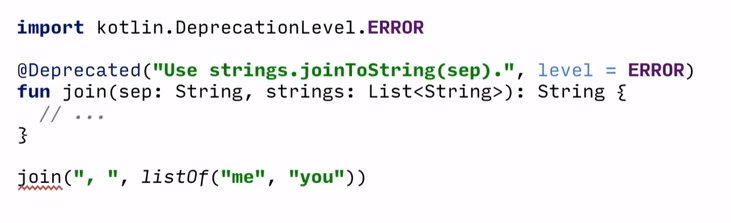
\includegraphics[scale=0.75]{DeprecationLevel.png}
  \caption{{\bfseries Errore a compile-time con \texttt{DeprecationLevel.ERROR}}}
  \label{deprecationError}
\end{figure}

\begin{figure}[ht]
  \centering
  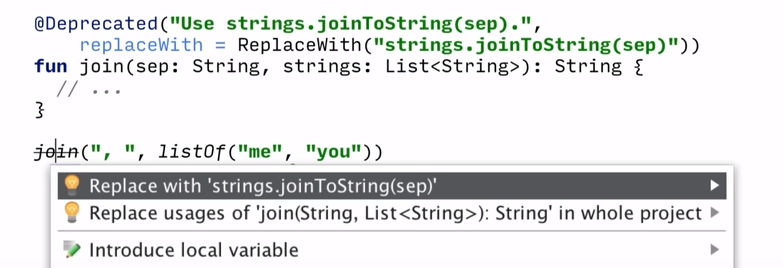
\includegraphics[scale=0.75]{DeprecationReplaceWith.png}
  \caption{{\bfseries Sostituzione a livello di IDE grazie al parametro \texttt{ReplaceWith}}}
  \label{deprecationWarning}
\end{figure}


Le annotazioni possono accettare come parametri soltanto tipi primitivi, stringhe, enumerazioni, riferimenti di classe, e array. La sintassi per specificare argomenti di annotazioni è leggermente diversa da Java.\\
Per specificare una classe come argomento di annotazione, è necessario inserire "\texttt{::class}" dopo il nome della classe, in questo modo:\\

\begin{lstlisting}[caption={Definizione di una annotazione personalizzata}, captionpos=b, label={lst:exAmpleAnnotCust}, language=Kotlin]
@MyAnnotation(MyClass::class)
\end{lstlisting}

Gli argomenti di annotazione devono essere noti al momento della compilazione, quindi se si intende utilizzare una proprietà come argomento di annotazione, è necessario contrassegnarla con il modificatore "\texttt{const}" (quindi deve essere inizializzata con valori di tipi primitivi o \texttt{String}), che riferisce al compilatore che la proprietà è una costante a compile-time.\\

\subsection{Coroutines}
Alcune API si servono di operazioni di tipo long-running (ad esempio operazioni di network IO, file IO, lavori intensivi su CPU o GPU, ecc.) e richiedono che il chiamante blocchi la propria esecuzione fino a quando esse non giungono al termine. Le {\em Kotlin Coroutines} forniscono un modo per evitare di eseguire manualmente blocchi sui thread e sostituire questa pratica con un'operazione più economica e controllabile: la sospensione di una coroutine.\\
Esse, infatti, semplificano la programmazione asincrona inserendo la logica della compilazione thread-safe nelle librerie: la logica del programma può essere espressa sequenzialmente in una coroutine, e la libreria sottostante intuirà l'asincronia in maniera trasparente. La libreria può wrappare parti rilevanti del codice utente in callback, sottoscrivere eventi rilevanti, schedulare l'esecuzione su thread diversi (o anche macchine diverse), lasciando che il codice rimanga semplice ed intuitivo come se fosse eseguito in sequenza. La sospensione di Coroutine è quasi gratuita: non è necessario alcun switch di contesto o qualsiasi altro coinvolgimento del sistema operativo. Molti meccanismi asincroni disponibili in altri linguaggi possono essere implementati ad hoc come librerie usando le coroutines di Kotlin: per fare alcuni esempi, si parla delle {\em async/await} di C\# e JavaScript, {\em channels} e {\em select} da Go, e {\em generator/yield} da C\# e Python.\\
Le Coroutines sono state la più grande novità nella release Kotlin v1.1 ed hanno suscitato molto entusiasmo all'interno della community a causa delle loro potenzialità. Tuttavia, sono un meccanismo ancora in fase sperimentale, che avrà la sua versione stabile solo con Kotlin v1.2.\\
Riassumendo, le coroutines si basano sull'idea di sospendere certe funzioni: quelle che possono bloccare l'esecuzione del programma nel momento in cui vengono chiamate e farla proseguire dopo aver terminato l'esecuzione del proprio compito: queste cosiddette "{\em suspending functions}" o funzioni di sospensione sono contrassegnate dalla parola chiave \texttt{suspend} e possono accettare parametri di ingresso e restituire valori in uscita allo stesso modo delle normali funzioni, ma possono essere chiamate solo all'interno di altre funzioni di sospensione o all'interno di una coroutine (d'altra parte, la libreria può decidere di procedere senza sospensione se il risultato della chiamata in questione è già disponibile); ciò significa che non è possibile invocarle in qualunque parte all'interno del codice, ma deve esserci una funzione circostante che costruisca la coroutine e fornisca il contesto richiesto per farlo. Una funzione di sospensione viene dichiarata con la seguente sintassi:\\

\begin{lstlisting}[caption={Definizione di una funzione di sospensione}, captionpos=b, label={lst:exAmpleSusp}, language=Kotlin]
suspend fun mySuspendingFunction(someParam: Int): Boolean {
    /* ... */
}
\end{lstlisting}

Un esempio semplificato di funzione \texttt{async} (disponibile nelle libreria \texttt{kotlinx.coroutines}) che permetta di fare chiamate a funzioni di sospensione è il \ref{lst:exAmpleAsync}:\\

\begin{lstlisting}[caption={Semplificazione della definizione della funzione di libreria \texttt{async}}, captionpos=b, label={lst:exAmpleAsync}, language=Kotlin]
fun <T> async(block: suspend () -> T)
\end{lstlisting}

Come si può notare, nell'esempio \ref{lst:exAmpleAsync}, \texttt{async} è una normale funzione (non di sospensione), ma il parametro "\texttt{block}" ha un function type con il modifier \texttt{suspend}: questo significa che quando viene passata un lambda a questa funzione, si tratterà di una lambda di sospensione, che permetterà di chiamare una funzione di sospensione al suo interno, nel seguente modo:\\

\begin{lstlisting}[caption={Utilizzo della funzione \texttt{async}}, captionpos=b, label={lst:exAmpleAsyncCall}, language=Kotlin]
async {
    mySuspendingFunction(someParam)

    /*...*/
}
\end{lstlisting}

Per arricchire l'esempio, la funzione \texttt{await} può essere una funzione di sospensione (quindi invocabile da un blocco \texttt{async{}}) che sospende una coroutine fino a quando non viene eseguito un certo tipo di computazione e restituisce il risultato:\\

\begin{lstlisting}[caption={Combinazione \texttt{async / await}}, captionpos=b, label={lst:exAmpleAwait}, language=Kotlin]
async {
    val resultOfAwait = computation.await()

    /*...*/
}
\end{lstlisting}

Discutendo del funzionamento interno, le coroutines sono interamente implementate attraverso una tecnica di compilazione (non è richiesto alcun supporto dal lato VM o OS) e la sospensione funziona tramite la trasformazione di codice. Fondamentalmente, ogni funzione di sospensione viene trasformata in una State Machine dove gli stati corrispondono alle chiamate di sospensione. Appena prima di una sospensione, lo stato successivo viene memorizzato in un campo di una classe generata dal compilatore insieme a variabili locali rilevanti e, una volta ripresa quella coroutine, le variabili locali vengono ripristinate e la macchina a stati procede dallo stato immediatamente successivo alla sospensione. Una coroutine sospesa può essere memorizzata e passata come un oggetto che mantiene lo stato di sospensione e le variabili locali. Il tipo assegnato a tali oggetti è \texttt{Continuation} e la trasformazione complessiva del codice citata corrisponde allo stile {\em Continuation-passing} proprio della programmazione funzionale. Di conseguenza, le funzioni di sospensione accettano in ingresso un ulteriore parametro di tipo \texttt{Continuation} in modo trasparente.\\

Nel contesto Android, le coroutine risultano molto utili, in quanto ci si può trovare molto facilmente ad utilizzare del codice asincrono, soprattutto lavorando con la GUI. Un esempio pragmatico di utilizzo di coroutines può essere rappresentato dal caricamento asincrono di due immagini (magari pesanti) all'interno di due differenti \texttt{View}:\\

\begin{lstlisting}[caption={Utilizzo di funzioni di libreria per Coroutines in Android}, captionpos=b, label={lst:exAmpleAsyncView}, language=Kotlin]
val first = loadImageAsync("green")
val second = loadImageAsync("red")
overlay(first.await(), second.await())
fun loadImageAsync(name: String) = async { /* ... */ }
\end{lstlisting}

La popolare libreria Anko, di cui si discuterà in seguito, fornisce molte soluzioni per implementare coroutines in maniera efficiente ed intuitiva in ambiente Android.\\

\section{Librerie}
Nonostante il linguaggio Kotlin si presti particolarmente a portare maggior fluidità e concisione nella programmazione di applicazioni Android, esistono diverse librerie che permettono di semplificare in maniera ancora superiore certe fasi dello sviluppo e certe caratteristiche dell'applicazione. Alcune di queste sono state sviluppate prima ancora che Kotlin ottenesse il titolo di linguaggio ufficialmente supportato da Google, quindi, una volta avvenuto l'annuncio al Google I / O 2017, hanno subito, insieme al linguaggio stesso una considerevole impennata nell'utilizzo da parte degli sviluppatori\\
Di seguito verranno menzionate le librerie più popolari e significative per lo sviluppo di sistemi Android; tuttavia, si consideri il fatto che, essendo Kotlin un linguaggio molto giovane ed ufficializzato da poco per la programmazione Android, queste ultime sono in continua e inesorabile espansione, pertanto verranno sicuramente ampliate e migliorate nel corso dei prossimi mesi e anni.\\

\subsection{Kotlin Android Extensions}
Questa libreria (a cui ci si riferisce anche con l’acronimo {\bfseries KAE}) non è più considerata tale circa dall'avvento di Kotlin v1.0, in quanto integrata automaticamente all'interno delle dipendenze Gradle per la compilazione di progetti Kotlin. Si tratta di una valida ed economica alternativa alla popolare Butter Knife (scritta in Java ed utilizzata soprattutto per effettuare view-binding semplificato): essendo un plugin integrato nel compilatore Kotlin non richiede aggiuntivo overhead a runtime.\\
L'import all'interno di un file Kotlin viene effettuato tipicamente in maniera automatica da Android Studio, aggiungendo le linee di codice definite nell'esempio \ref{lst:exAmpleImportKAE}:\\

\begin{lstlisting}[caption={Import delle Kotlin Android Extensions}, captionpos=b, label={lst:exAmpleImportKAE}, language=Kotlin]
import kotlinx.android.synthetic.main.<layout>.*      //Oppure
import kotlinx.android.synthetic.main.<layout>.view.*
\end{lstlisting}

L'utilizzo di queste Extensions risulta molto intuitivo ed immediato. Si parla di proprietà {\em synthetic} quando ci si riferisce a quella parte della libreria che permette di effettuare il view-binding in stile Butter Knife: per effettuare binding è sufficiente chiamare (ovviamente, successivamente all'invocazione della funzione \texttt{setContentView}) le componenti della view utilizzando semplicemente il loro resource-id definito nel rispettivo file xml; il compilatore effettuerà implicitamente il binding, e sarà possibile riferirsi al componente senza necessità di invocare la funzione \texttt{findViewById} (che richiederebbe la definizione di una nuova variabile da associare al componente).\\

\begin{lstlisting}[caption={Utilizzo delle proprietà synthetic di KAE}, captionpos=b, label={lst:exAmpleKAE}, language=Kotlin]
import android.support.v7.app.AppCompatActivity
import android.os.Bundle
import kotlinx.android.synthetic.main.activity_main.*

class MainActivity : AppCompatActivity() {
  override fun onCreate(savedInstanceState: Bundle?) {
    super.onCreate(savedInstanceState)
    setContentView(R.layout.activity_main)
    text_view_helloworld.text = "My Text!" //Riferimento diretto all'ID xml
  }
}
\end{lstlisting}

\subsection{Anko}
Anko è una DSL library (Domain-Specific Language) per Android scritta interamente in Kotlin, sviluppata e gestita da JetBrains sotto licenza Apache 2.0, annunciata al pubblico sul sito ufficiale di Kotlin l'8 aprile 2015, ed è stata pensata per aiutare a costruire l'interfaccia utente di applicazioni Android.\\ Tradizionalmente, le view in Android vengono espresse come layout XML. Uno svantaggio di esprimere interamente le componenti della View in file di questo tipo riguarda il fatto che ciò comporta molto spesso duplicazione di codice in varie parti dell'applicazione; codice che non viene riutilizzato. A runtime, questi file XML vengono trasformati nella rappresentazione Java della View, utilizzando in maniera inutile CPU e batteria. La libreria Anko permette di definire i file di layout all'interno di file .kt: un'\texttt{Activity} o un \texttt{Fragment} (o anche come \texttt{AnkoComponent}, un file esterno di Kotlin che rappresenta la vista). Si propone un esempio di come la libreria Anko fornisca wrapper per le API Android classiche in una struttura DSL-like, definendo una funzione di estensione che costruisce un \texttt{AlertDialog} che mostra un messaggio e due opzioni: procedere oltre o interrompere l'operazione.\\

\begin{lstlisting}[caption={Utilizzo di Anko per costruire un \texttt{AlertDialog}}, captionpos=b, label={lst:exAmpleAnko}, language=Kotlin]
fun Activity.showAreYouSureAlert(process: () -> Unit) {
  alert(title = "Are you sure?", message = "Are you really sure?") {
      	positiveButton("Yes") { process() }
      	negativeButton("No") { cancel() }
  }
}
\end{lstlisting}
Nello snippet di codice dell'esempio \ref{lst:exAmpleAnko} sono presenti tre differenti espressioni lambda: la prima è il terzo argomento della funzione \texttt{alert} e le altre due vengono passate come argomenti a \texttt{positiveButton} e \texttt{negativeButton}. Il receiver della prima lambda (esterna) è di tipo \texttt{AlertDialogBuilder}.\\
Di seguito sono riportate le dichiarazioni dei membri utilizzati nell'esempio \ref{lst:exAmpleAnko}:\\
\\

\begin{lstlisting}[caption={Definizione di funzioni di libreria Anko}, captionpos=b, label={lst:exAmpleAnkoDef}, language=Kotlin]
fun Context.alert(
  message: String,
  title: String,
  init: AlertDialogBuilder.() -> Unit
)

class AlertDialogBuilder {
  fun positiveButton(text: String, callback: DialogInterface.() -> Unit)
  fun negativeButton(text: String, callback: DialogInterface.() -> Unit)
  /* ... */
}
\end{lstlisting}

Come si può notare, vengono aggiunti due pulsanti alla \texttt{AlertDialog} di avviso. Se l'utente fa clic sul pulsante "\texttt{Yes}" verrà chiamata la azione \texttt{process}, altrimenti verrà invocato \texttt{cancel} (il quale è un membro dell'interfaccia \texttt{DialogInterface}, viene quindi chiamato su un receiver implicito di questa lambda) e l'operazione verrà annullata.\\
Tuttavia, la novità più importante della libreria Anko è fornire un DSL che funga da alternativa completa alla definizione di un layout in XML. L'idea è quella di sostituire le definizioni di layout XML con del codice Kotlin, senza dover costruire il layout in un senso veramente programmatico. La libreria Anko si pone come obiettivo quello di rappresentare una alternativa non solo completa, ma anche credibile e conveniente alla scrittura di file XML: fornisce wrapper molto concisi ed intuitivi, che con poche linee di codice possono creare una UI che in XML richiederebbe molto più sforzo implementativo. Negli esempi \ref{lst:exAmpleAnkoXML}, \ref{lst:exAmpleAnkoKt} e \ref{lst:exAmpleAnkoAnko} si mostreranno tre diverse implementazioni di una UI Android fornita semplicemente di un \texttt{LinearLayout}, che contenga una \texttt{EditText} ed un \texttt{Button}: utilizzando, nell'ordine, XML, Kotlin ed Anko.\\

\begin{lstlisting}[caption={Interfaccia definita in un file XML}, captionpos=b, label={lst:exAmpleAnkoXML}, language=XML]
<LinearLayout xmlns:android="http://schemas.android.com/apk/res/android"
    android:orientation="vertical"
    android:layout_width="match_parent"
    android:layout_height="match_parent">
    <EditText
        android:layout_width="match_parent"
        android:gravity="center"
        android:text="@string/empty_todos_message"
        android:layout_weight="7"
        android:layout_height="wrap_content" />
    <Button
        android:layout_width="match_parent"
        android:layout_weight="1"
        android:text="Say Hello"
        android:layout_height="0dp" />
</LinearLayout>
\end{lstlisting}

\begin{lstlisting}[caption={Interfaccia definita programmaticamente con un blocco di codice Kotlin semplice}, captionpos=b, label={lst:exAmpleAnkoKt}, language=Kotlin]
val act = this
val layout = LinearLayout(act)
layout.orientation = LinearLayout.VERTICAL
val name = EditText(act)
val button = Button(act)
button.text = "Say Hello"
button.setOnClickListener {
  Toast.makeText(act, "Hello, ${name.text}!", Toast.LENGTH_SHORT).show()
}
layout.addView(name)
layout.addView(button)
\end{lstlisting}

\begin{lstlisting}[caption={Interfaccia definita programmaticamente utilizzando i wrapper della libreria Anko}, captionpos=b, label={lst:exAmpleAnkoAnko}, language=Kotlin]
verticalLayout {
    val name = editText()
    button("Say Hello") {
      onClick { toast("Hello, ${name.text}!") }
    }
}
\end{lstlisting}

Uno dei benefici fondamentali che può portare l'uso di questa libreria è sicuramente quello di avere "tutto in un unico posto", citando il team di JetBrains: invece di dividere i layout in parti statiche (XML) e dinamiche e poi cercare di fare in modo di legarle insieme, Anko dà la possibilità di scrivere parti di view e di controllo usando solamente il linguaggio Kotlin, con il vantaggio di rendere il tutto più conciso e leggibile e consentendo un più semplice riutilizzo.\\
Anko fornisce anche ulteriori wrapper ed espedienti di varia natura, spaziando in molte funzionalità di Android: possiede diversi shortcut per i \texttt{Service}, qualificatori per la configurazione dell'interfaccia (ad esempio \texttt{screenSize}, \texttt{orientation}, ecc.), wrapper per implementare task asincroni, e una vasta gamma di funzioni utili per rendere più immediata l'interazione con SQLLite.\\

\subsection{Kotter Knife}
La libreria Kotter Knife fornisce funzionalità molto simili alle Kotlin Extension per Android: fondamentalmente fa wrapping di operazioni di view-binding. Tuttavia, risulta più simile a Butter Knife (come il nome stesso suggerisce); presenta, inoltre, feature aggiuntive, come il binding di listeners e risorse, non presenti in Kotlin Android Extensions. Di seguito si riporta un blocco di codice (\ref{lst:exAmpleKotterKt}) che riporta due esempi di utilizzo di Kotter Knife:\\

\begin{lstlisting}[caption={Due esempi di uso di Kotter Knife con Kotlin}, captionpos=b, label={lst:exAmpleKotterKt}, language=Kotlin]
val btnSend: Button by bindView(R.id.btn_send)
btnSend.setOnClickListener( { view -> Log.d("MainActivity", "onClick: send") } )

//Oppure, combinando Kotter Knife con la libreria KAE kotlinx.android.synthetic

import kotlinx.android.synthetic.activity_main.*
btn_send.setOnClickListener( { view -> Log.d("MainActivity", "onClick: send") } )
\end{lstlisting}

\subsection{Altre Librerie}
Come accennato, esistono attualmente moltissime librerie scritte in Kotlin che supportano la programmazione Android, e risultano in continua espansione. Si riportano di seguito le più significative tra quelle considerate "minori".\\

\begin{itemize}
  \item {\bfseries KAndroid} - Questa libreria (con licenza Apache 2.0) contiene extension s che forniscono utilities che spaziano su tutto il framework Android, con l'obiettivo di diminuire il boilerplate. Tra le feature, si citano il view-binding, delle estensioni per \texttt{SeekBar} e \texttt{SearchView}, utilities per il Logging, gli \texttt{Intent} e la gestione di Thread.
  \item {\bfseries Kovenant} - Non è una libreria Android-specific (con licenza MIT), ma merita una menzione, in quanto fornisce feature che vanno dal semplificare uso di Task e callback, all'interazione con la User Interface.
  \item {\bfseries Fuel} - Una libreria utile per lavorare con il protocollo HTTP su Android: supporta chiamate bloccanti e asincrone, il download e upload di file, Gson ed API routing.
  \item {\bfseries Bubble} - Una libreria molto utile che fornisce informazioni sull'orientazione dello schermo ogni qualvolta che una rotazione viene identificata.
  \item {\bfseries TornadoFX} - Si tratta di una libreria non Android-Specific che fornisce API Kotlin per interagire con il framework JavaFX.\\
\end{itemize}

\section{Analisi Prestazioni}
In generale, chiedersi quali linguaggi siano "più veloci" di altri non è esattamente l'approccio giusto per un'analisi concreta. In questo caso, siccome il byte-code generato da Kotlin è fondamentalmente identico a quello generato dal codice Java, non esiste una differenza consistente e misurabile. Inoltre, il codice che si scrive molto spesso determina la "velocità" del proprio programma in misura molto maggiore rispetto a qualsiasi efficienza acquisita eseguendo la propria implementazione di un costrutto utilizzando un linguaggio piuttosto che un altro.\\
Kotlin non introduce alcuna semantica runtime aggiuntiva rispetto a Java: non presenta meta-programmazione, per esempio e anche Groovy, che invece ne possiede, è estremamente vicino alle prestazioni del Java puro.
C’è da aggiungere che il linguaggio Kotlin è fondamentalmente focalizzato su Android: è stato scritto dalle stesse persone che hanno creato ambienti di progettazione integrata molto popolari (IDE come IntelliJ IDEA, CLion e altre), quindi il suo background proviene da professionisti del settore mobile che stavano cercando di risolvere problemi specifici.\\

\subsection{Prestazioni di Compilazione}
Analizzando le prestazioni in campo Android, ci si pone la seguente domanda: se si converte un'applicazione da Java a Kotlin, questa impiegherà più tempo per compilare?\\
La conversione di un'applicazione Android da Java ad un codice sorgente scritto al 100\% in Kotlin comporta sicuramente una riduzione sostanziale del code-base, tuttavia molti sviluppatori affermano di non voler iniziare il cambiamento di linguaggio di programmazione in quanto preoccupati dei tempi di compilazione: si tratta certamente di una preoccupazione valida.\\
La compilazione di codice Kotlin non comporta un overhead in termini di tempi di compilazione percepibile, anzi, in molti casi Kotlin fornisce feature che permettono di eseguire build anche più rapide rispetto a Java: le lambda Kotlin, ad esempio, risultano molto più "leggere" da compilare rispetto a quelle di Java 7; un'altra discriminante in questo caso è rappresentata dalle cosiddette {\em inline functions}, che permettono una compilazione più pulita, guadagnando rispetto a Java in termini di tempi di build. Inoltre, attivando il Gradle daemon (operazione possibile passando {\bfseries \texttt{--daemon}} come parametro a Gradle da riga di comando, oppure aggiungendo la riga "{\bfseries \texttt{org.gradle.daemon = true}}" al file \texttt{gradle.properties}), è possibile guadagnare in termini di prestazioni in ambito di build successive: la prima build richiederà la stessa quantità di tempo di quella effettuata senza utilizzare questo strumento, ma le esecuzioni successive aumenteranno considerevolmente in prestazioni. Il demone Gradle, infatti, riduce i tempi di build di una qualsiasi applicazione di oltre il 40\%.\\
Tuttavia, solitamente si compila dopo aver apportato modifiche a pochi file e le build incrementali avranno caratteristiche di performance diverse: le build incrementali hanno infatti un enorme impatto sui tempi di compilazione, specialmente per i progetti di grandi dimensioni.
Questo particolare tipo di build è stato aggiunto a Kotlin nella versione 1.0.2, ed è possibile abilitarle aggiungendo la riga "{\bfseries \texttt{kotlin.incremental = true}}" al file \texttt{gradle.properties} o usando un'opzione della riga di comando. Nella configurazione più comune (ovvero eseguendo build parziali con compilazione incrementale abilitata) Kotlin si compila tanto velocemente quanto Java, o leggermente di più.\\

\begin{figure}[ht]
  \centering
  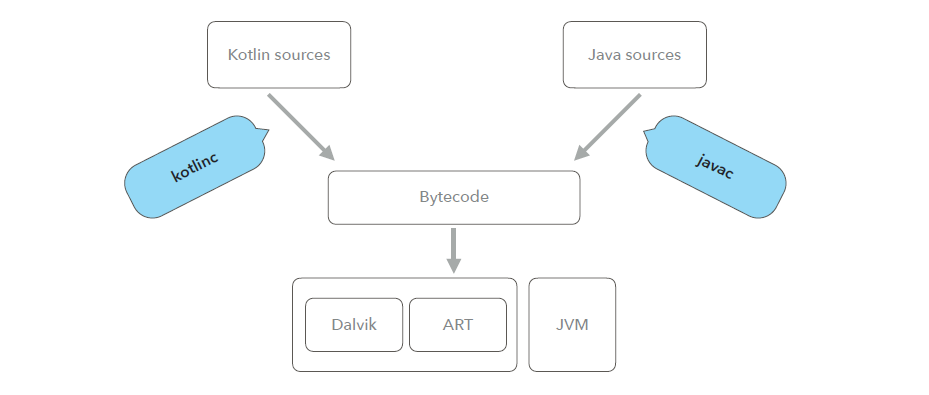
\includegraphics[scale=0.66]{KotlinCompiling.png}
  \caption{{\bfseries Schematizzazione del processo di compilazione}}
  \label{KotlinCompiling}
\end{figure}

\subsection{Conteggio dei metodi}
Questa problematica è spesso sottovalutata nella scelta dei linguaggi di programmazione da utilizzare, ma è molto importante, soprattutto in un ambito dalle risorse teoricamente limitate come quello dei sistemi mobile: quando 65.000 è il massimo dei metodi importabili in una applicazione, aggiungere una nuova libreria può risultare scoraggiante. Il cosiddetto problema del {\em method count} è stato, ad esempio, una discriminante nella scelta da parte di JetBrains di non utilizzare Scala come alternativa a Java (in quanto linguaggio che aggiunge un considerevole overhead in termini di method count), ma di sviluppare un nuovo linguaggio JVM. In generale è consigliato l'uso del tool {\bfseries ProGuard} per tagliare tutti i metodi non utilizzati; con questo tool, il method count di Kotlin su una generica applicazione Android risulta del 1.3\% rispetto al totale dei metodi presenti: pochissimi per un intero linguaggio.\\
Una discriminante in questo caso riguarda in particolare il modo in cui vengono implementate le lambda rispetto a Java 8, che è recentemente diventato disponibile in Android. In alcuni casi, Kotlin genera effettivamente un codice bytecode più efficiente attraverso l'uso di funzioni inline, il che significa che il codice è "allineato" alla linea di chiamata e il method count rimane così invariato. Di conseguenza, nel peggiore dei casi Kotlin, nello sviluppo di applicazioni Android, produce lo stesso numero di metodi di Java 8, nel caso migliore (e probabilmente medio) ancora più basso.\\

\subsection{Impatto sulle dimensioni e quantità di linee di codice}
Per quanto riguarda le dimensioni dei file apk generati da progetti scritti in Kotlin, si riscontra un leggero incremento: tipicamente, le applicazioni Kotlin risultano più pesanti di solo lo 0.6\% rispetto a quelle Java (anche qui utilizzando ProGuard). Diverso è il discorso riguardante le {\em lines-of-code}, infatti, come già discusso il linguaggio Kotlin porta una considerevole riduzione delle linee di codice: uno dei principi fondamentali della filosofia di Kotlin, infatti, è proprio la concisione, e questo si manifesta soprattutto scrivendo codice per Android. L'uso integrale di Kotlin all'interno della propria applicazione permette di ridurre, tipicamente, del 25\% il numero delle righe di codice impiegate per scriverla: un miglioramento decisamente notevole.\\

\subsection{Stabilità}
Un'altra preoccupazione manifestata dagli sviluppatori Java rispetto al passaggio al programmare in Kotlin è rappresentata dalla stabilità dell'applicazione. In questo caso, basta citare la filosofia Null-safety che Kotlin introduce: la produzione di crash da parte di un'applicazione dipende soprattutto dal programmatore, e in maniera decisamente minima dal linguaggio; tuttavia, Kotlin fornisce un sistema di tipi che previene in maniera sistematica gravi errori come le \texttt{NullPointerException} (che portano, appunto, al crash dell'applicativo), dunque aggiunge un ulteriore livello di stabilità rispetto a Java in questo senso.\\

    %% Direttive TeXworks:
% !TeX root = ../semprini_luca_tesi.tex
% !TEX encoding = UTF-8 Unicode
% !TEX program = arara
% !TEX TS-program = arara
% !TeX spellcheck = it-IT

\chapter{Analisi Conclusiva}\label{ch:conclusione}

\section{Situazione Attuale}
Allo stato attuale, il linguaggio Kotlin è in continua evoluzione. Per quanto riguarda l'ambito della piattaforma Android, fin dalle primissime release, Kotlin ha sempre avuto un appeal particolare nei confronti di molti sviluppatori: essendo stato progettato per rendere la progettazione di applicazioni più "divertente" rispetto all'utilizzo di Java, ha da subito riscosso un grande interesse nella community Java, ma non solo. Molte aziende e sviluppatori indipendenti hanno immediatamente optato per iniziare uno switch a livello di codice sorgente da Java a Kotlin, in quanto particolarmente attratti dalla filosofia e dalle funzionalità del linguaggio; tuttavia questa operazione ha rappresentato, a priori, un rischio, poiché il linguaggio era ancora molto giovane e soprattutto non supportato dal team di Google. Successivamente alla Google I / O del 17 maggio 2017, l'assunzione di Kotlin da parte di moltissime aziende come linguaggio principale in cui sviluppare le proprie applicazioni mobile ha subito un’impennata notevole, guidata dall’entusiasmo che ha contaminato gli sviluppatori Android a seguito dell'annuncio ufficiale alla conferenza.\\

Attualmente, ci sono moltissime aziende note che lo utilizzano in produzione: ad esempio, Pinterest è stata una delle prime compagnie a farne uso in maniera preponderante per la sua app Android. Un altro grande esempio è rappresentato dalla situazione di Basecamp: la compagnia americana fa già uso di Kotlin nel 100\% del codice sorgente della propria applicazione. Per mostrare altri esempi di aziende che si stanno affidando a Kotlin in questo ambito, si possono citare Trello, Netflix, Prezi, Hootsuite, NBC News Digital, e molte altre.\\

Un altro importante fatto da riportare riguarda le offerte di lavoro da parte di molte aziende: queste ultime stanno iniziando a richiedere competenze approfondite di linguaggio Kotlin per i loro posti di lavoro. Non solo, molte compagnie stanno iniziando a fare investimenti di denaro nella formazione dei propri dipendenti in modo da avere sviluppatori Kotlin.\\
Quindi, anche se Kotlin non è adottato nella maggior parte delle aziende per progettare applicazioni Android, vi sono già alcune compagnie che ne stanno facendo uso, le quali, durante la propria crescita, avranno sempre più bisogno di esperti di Kotlin. Molti sviluppatori indipendenti che avevano scommesso su un linguaggio appena annunciato come era Kotlin agli inizi, approfondendone e apprendendone le funzionalità più avanzate, hanno oggi facilmente trovato lavoro grazie a questa intuizione.\\

Inoltre, Kotlin risulta molto facile da imparare, sia per le sue caratteristiche sintattiche (che ricordano quelle di molti linguaggi esistenti e familiari per gli sviluppatori di applicazioni mobili, come Java, JavaScript e Groovy), sia per i tool di supporto all'apprendimento, come {\bfseries Kotlin-koans} \footnote{\url{https://github.com/Kotlin/kotlin-koans}}: un set di esercizi per familiarizzare il programmatore con la sintassi di Kotlin. Ogni esercizio viene creato come uno Unit-test che fallisce di default, e il compito dello "studente" è quello di modificare alcune parti di codice per permettere che il test abbia successo. È possibile utilizzare Koans online, direttamente all'interno di IntelliJ IDEA o Android Studio, o clonando il progetto da GitHub. Un altro tool molto utile in questo senso è il già citato convertitore "Java-to-Kotlin" e "Kotlin-to-Java", che permette al programmatore di iniziare a scrivere codice Kotlin a piccoli passi, inizialmente traducendo il proprio codice Java automaticamente in Kotlin, per imparare meglio la sintassi.\\
Sotto l'aspetto istruttivo, il team di Kotlin suggerisce anche numerose letture utili per familiarizzare con il linguaggio, come
Kotlin in Action \cite{kaction}, Kotlin for Android Developers \cite{leiva}, Programming Kotlin \cite{programmingKotlin} e altri.\\

Ad oggi, successivamente alla KotlinConf e dopo quasi 7 mesi dall'annuncio ufficiale di Kotlin come linguaggio first-class per Android al Google I / O, il numero di app sul Google Play Store implementate in Kotlin è più che raddoppiato: attualmente, oltre il 17\% dei progetti in Android Studio 3.0 utilizza Kotlin \cite{ktUpdateAndroidDevBlog}, e la tendenza è in continuo aumento. Per considerare l'importanza dell'annuncio da parte di Google di supportare Kotlin come linguaggio first-class, si noti la figura \ref{GoogleInterest}.\\
\\
\\

\begin{figure}[ht]
  \centering
  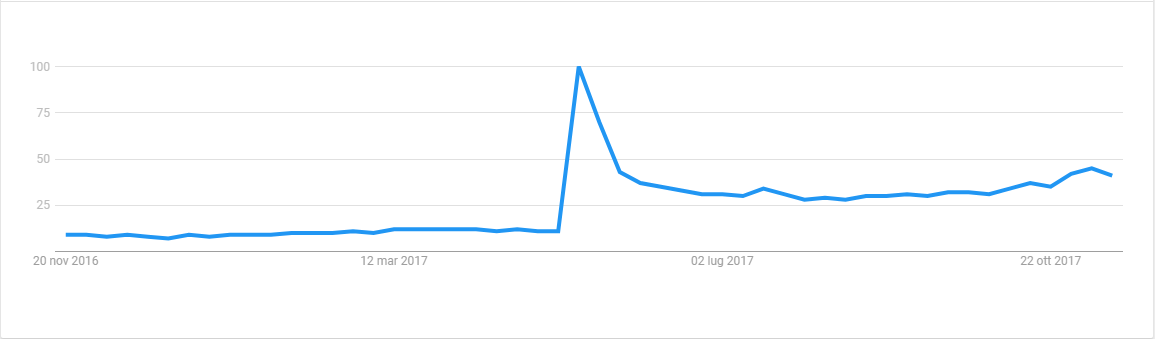
\includegraphics[scale=0.5]{GoogleInterest.png}
  \caption{{\bfseries Interesse nel tempo per Kotlin stimato da Google Trends}}
  \label{GoogleInterest}
\end{figure}

Come si può notare, l'impennata della curva di interesse riportata nel grafico della figura \ref{GoogleInterest} corrisponde esattamente con l'annuncio del 17 maggio 2017; l'interesse va successivamente calando, fino ad assestarsi su un valore comunque di molto superiore a quello che possedeva prima del Google I / O, ma risulta comunque in continua ascesa. Anche le date del 3 e 4 novembre 2017 contribuiscono al grafico: la leggera risalita che si può notare sulla parte destra del grafico, infatti, corrisponde proprio alla KotlinConf di San Francisco.\\

\section{Prospettive future per Kotlin}

Secondo un rapporto \cite{realmReport} pubblicato da Realm \cite{realm} (un famoso fornitore di un popolare e indipendente database mobile in-app) pubblicato il 25 settembre 2017, la tendenza all'adozione di Kotlin è aumentata molto rapidamente e potrebbe superare Java nel dicembre del 2018, ovvero circa 17 mesi dopo che Google ha annunciato il supporto ufficiale al linguaggio di JetBrains e 2 anni e mezzo dopo che Kotlin ha raggiunto la v1.0; per fare un confronto, per quanto riguarda il sistema iOS, ci sono voluti solo 14 mesi dopo il rilascio di Swift v1.0 prima di raggiungere lo stesso picco rispetto ad Objective-C, ma ovviamente si è trattato di una situazione molto diversa: Swift è, infatti, un linguaggio proprietario di Apple, pensato esclusivamente per sviluppare applicazioni iOS.\\

I risultati del rapporto si basano su un'analisi del comportamento di oltre 100.000 sviluppatori che utilizzano il database di Realm nelle loro applicazioni. Il DB mobile è attualmente installato su oltre 3,5 miliardi di applicazioni iOS e Android, tra cui Starbucks, SAP, eBay, Intel e Alibaba. Il rapporto è il primo di una serie trimestrale pianificata, ha spiegato Paul Kopacki, VP del marketing di Realm.\\
La società ha compilato i dati sullo sviluppo di applicazioni mobili che utilizzano il loro database da agosto 2015 e questa prima edizione del Realm Report si è concentrata sui linguaggi di programmazione più popolari che gli sviluppatori utilizzano per creare applicazioni mobili e ha riscontrato quanto segue.\\

\begin{figure}[ht]
  \centering
  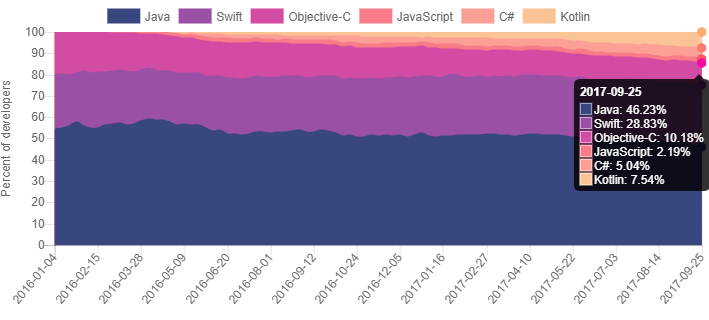
\includegraphics[scale=0.60]{languages.png}
  \caption{{\bfseries Linguaggi di programmazione per sistemi mobile più popolari secondo Realm}}
  \label{languages}
\end{figure}

Come si può notare dalla tendenza mostrata dal grafico in figura \ref{languages}, Java sta perdendo il mindshare (appetibilità) degli sviluppatori ed anche velocemente: la percentuale di applicazioni Android create utilizzando Java è diminuita del 6.1\% e negli ultimi quattro mesi è scesa dal 50.7\% al 46.2\% delle app complessive, e questo significa che l'adozione di Kotlin come principale linguaggio con cui programmare applicazioni Android sta esplodendo: il numero di applicazioni create utilizzando Kotlin, infatti, è cresciuto del 125\%. Un altro dato interessante fornito da questo rapporto riguarda applicazioni già esistenti scritte in Java: il 20\% delle applicazioni Kotlin costruite dopo la conferenza Google I / O erano state precedentemente costruite con Java, il che significa che non c'è stata solo un'esplosione del linguaggio per quanto riguarda i nuovi progetti, ma che si sta operando uno switch di linguaggio di programmazione anche nelle applicazioni già consolidate ed inizialmente progettate in Java.\\
Nonostante il supporto a Java 8 dalla versione 3.0 di Android Studio, gli sviluppatori stanno mostrando sempre più interesse per il nuovo linguaggio proposto da JetBrains. Di seguito si riporta un grafico reso disponibile da Realm, che fotografa la situazione di Kotlin e Java in due momenti ravvicinati, ma molto differenti.\\

\begin{figure}[ht]
  \centering
  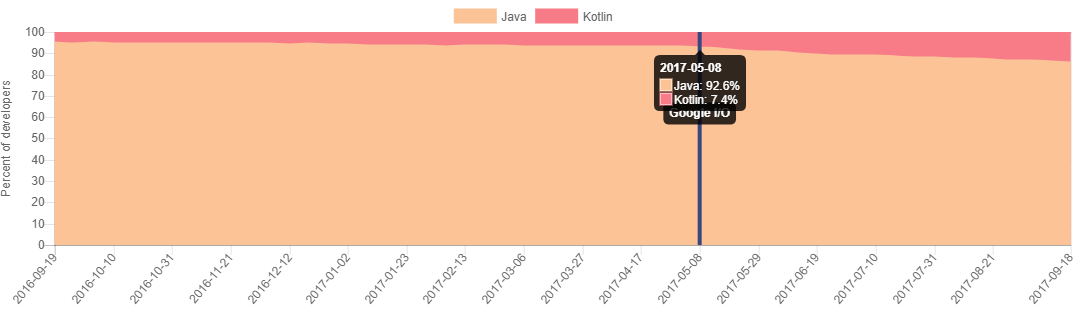
\includegraphics[scale=0.4]{downloadGIO.png}
  \caption{{\bfseries Utilizo di Kotlin e Java in applicazioni Android prima del Google I / O}}
  \label{gio}
\end{figure}

\begin{figure}[ht]
  \centering
  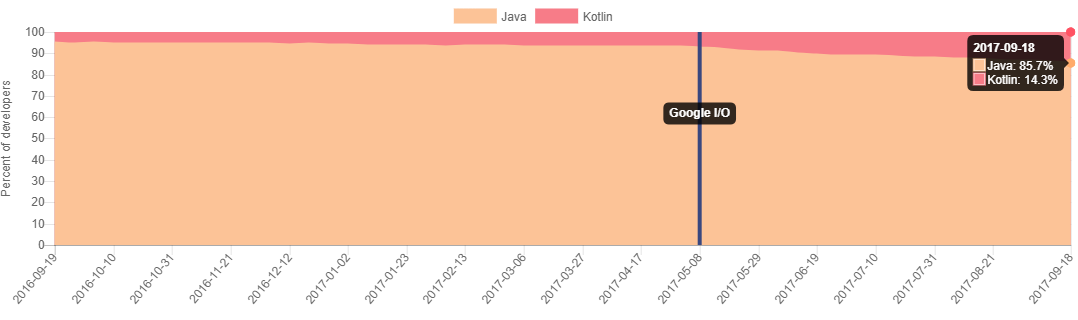
\includegraphics[scale=0.4]{downloadNow.png}
  \caption{{\bfseries Utilizo di Kotlin e Java in applicazioni Android in data 18 settembre 2017}}
  \label{now}
\end{figure}

La figura \ref{gio} riporta i dati dell'utilizzo di Java e Kotlin da parte degli sviluppatori in data 8 maggio 2017, quindi pochi giorni prima dell'annuncio del supporto ufficiale di Google; la figura \ref{now}, invece, mostra quanto velocemente sia accresciuto l'interesse verso il nuovo linguaggio da parte dei programmatori in pochi mesi: dal 7.4\% di utilizzo è, infatti, passato al 14.3\%.\\

Per quanto riguarda le proiezioni future, il rapporto di Realm prevede, come anticipato, che Kotlin supererà Java molto presto. Sulla base dei dati, questo avverrà circa nel mese di dicembre 2018. Realm è abbastanza ottimista sul futuro di Kotlin e non solo, il rapporto afferma, infatti, che "presto, gli sviluppatori Android che non hanno competenze di Kotlin rischieranno di essere considerati come dinosauri" \cite{realmReport}.\\
Ciò significa che gli sviluppatori (quantomeno in ambito Android) che rimarranno ancorati sul linguaggio Java correranno il rischio di diventare obsoleti, per cui le possibilità di trovare un lavoro come programmatori di applicazioni Android saranno ridotte poiché sarà necessaria la conoscenza di un linguaggio più moderno tra i requisiti. Inoltre, Realm prevede un grande futuro per Kotlin anche in altri ambienti come quello server, dove, anche qui, potrebbe arrivare a sostituire Java; con gli ultimi annunci da parte di JetBrains, infine, sta cominciando sempre più a farsi strada la possibilità di un utilizzo di Kotlin su progetti multi-piattaforma, quindi anche su sistemi iOS e servizi web front-end.
Si noti, dunque, un ulteriore grafico reso disponibile da Realm, che riporta, sulla base di una proiezione statistica, la aspettativa di crescita di utilizzo del linguaggio Kotlin nei sistemi Android nei prossimi mesi.\\

\begin{figure}[ht]
  \centering
  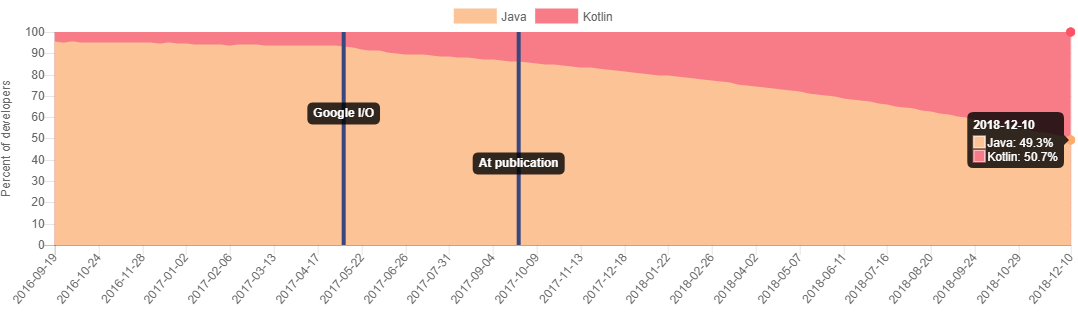
\includegraphics[scale=0.4]{downloadProjected.png}
  \caption{{\bfseries Proiezione del grafico precedente per l'utilizzo di Kotlin rispetto a Java in applicazioni per la piattaforma Android}}
  \label{projected}
\end{figure}

Il grafico in figura \ref{projected} mostra come, sulla base dei dati riportati da Realm e su una proiezione statistica, Kotlin potrebbe soppiantare Java in termini di percentuale di utilizzatori in poco più di un anno dalla pubblicazione del primo rapporto (data contrassegnata dalla linea verticale con etichetta "At publication"). Ovviamente si tratta di una proiezione ottimistica, che prevede che l'entusiasmo dei programmatori nei confronti del nuovo linguaggio cresca con lo stesso andamento con cui è cresciuto nelle settimane immediatamente successive al Google I / O. Tuttavia, non è una proiezione inverosimile, in quanto l'appetibilità di Kotlin agli occhi degli sviluppatori è sicuramente un dato di fatto, e la popolarità del linguaggio sta inesorabilmente crescendo. Infine, il Realm Report non è il solo recente rapporto del settore a notare un aumento della popolarità di Kotlin: Redmonk, Tiobe e RebelLabs hanno riconosciuto il suo impatto, specialmente su Java, che era una volta l'unico linguaggio disponibile per gli sviluppatori Android.

    % %% Direttive TeXworks:
% !TeX root = ../semprini_luca_tesi.tex
% !TEX encoding = UTF-8 Unicode
% !TEX program = arara
% !TEX TS-program = arara
% !TeX spellcheck = it-IT

%% Direttive Arara:
% arara: pdflatex: { shell: yes, synctex: yes, action: batchmode, options: "-halt-on-error -file-line-error-style" }
% arara: frontespizio
%! arara: bibtex
% arara: pdflatex: { shell: yes, synctex: yes, action: batchmode, options: "-halt-on-error -file-line-error-style" }
% arara: pdflatex: { shell: yes, synctex: yes, action: nonstopmode, options: "-halt-on-error -file-line-error-style" }

\appendix

% TODO


    \backmatter
    %% Direttive TeXworks:
% !TeX root = ../maltoni_niccolo_tesi.tex
% !TEX encoding = UTF-8 Unicode
% !TEX program = arara
% !TEX TS-program = arara
% !TeX spellcheck = it-IT

\nocite{IJIR5491}
\nocite{Takeuchi:2013:JIM:2481268.2481278}
\printbibliography[heading=bibintoc]

    % \listoffigures
    % \listoftables
    % \input{tex/backmatter/ringraziamenti.tex}
\end{document}
